\documentclass[11pt,a4paper,oneside,ngerman,appendixprefix=true,listof=chapterentry]{report}
\usepackage[ngerman]{babel}
%\usepackage[latin1]{inputenc}
\usepackage[utf8]{inputenc}
\usepackage{bibgerm} 
\usepackage[german]{varioref}
\usepackage{hyperref}
\usepackage{url}
\usepackage[table]{xcolor}
\usepackage{textcomp}
\usepackage{listings}
\usepackage{mcode}
\usepackage{lipsum}
\usepackage{amsmath} 
\usepackage{chngpage}
\usepackage[titletoc,toc]{appendix}
\usepackage{acronym}
\usepackage{array}
\usepackage{calc,layouts}
\usepackage{float}
\usepackage{dcolumn}
\usepackage[section]{placeins}
\usepackage[hang]{caption}
\usepackage{subcaption}
\usepackage{graphicx}
\usepackage{tabularx}
\usepackage{multirow}
\usepackage{rotating}
\usepackage{units}
\usepackage{wrapfig}
\usepackage{pdfpages}
\usepackage{geometry}
\usepackage[babel,german=quotes]{csquotes}
\usepackage[scaled]{helvet}
\usepackage[onehalfspacing]{setspace}
\geometry{a4paper, top=25mm, left=25mm, right=25mm, bottom=30mm,headsep=10mm, footskip=12mm}
\begin{document}
\pagenumbering{arabic}
\begin{titlepage}
\begin{center}
\LARGE{Bachelor's Thesis}\vspace{0.5cm}\\
\LARGE{\textbf{Aufbau einer Schnittstelle zwischen MATLAB und einer Wetterstation über MODBUS\\ Development of a MATLAB gateway to a hardware weather station via MODBUS}}\vspace{0.5cm}\\
verfasst von\vspace{0.5cm}\\
Andreas Henneberger\\
\textbf{Matr.Nr. 2647351}\vspace{0.5cm}\\
eingereicht am\vspace{0.25cm}\\
\LARGE{\textbf{Lehrstuhl für Energiewirtschaft und Anwendungstechnik\\Technische Universität München,}}\vspace{0.25cm}\\
bei\vspace{0.25cm}\\
\textbf{Prof. Dr. rer. nat. Thomas Hamacher}\vspace{0.5cm}\\
Betreuer: Dipl.-Ing. Christian Kandler und Dipl.-Ing. Patrick Wimmer
\end{center}



\end{titlepage}

\begin{abstract}
Ziel dieser Arbeit ist es eine Schnittstelle zwischen MATLAB und einer Wetterstation aufzubauen, um darüber Prognosedaten für ein integriertes Energiemanagementsystem bereitzustellen. Diese Informationen sollen dazu dienen die Planungen des Managementsystems im Smart-Micro-Grid hinsichtlich Lastverläufe und Energieerzeugung zu vereinfachen bzw. zu präzisieren. Die Datenbereitstellung erfolgt über einen Langwellenempfänger, dessen Register über eine MODBUS Kommunikation abgerufen werden können. Die meisten gelieferten Werte weisen eine zeitliche Auflösung von 6 Stunden auf. Da das Managementsystem jedoch umso genauer arbeiten kann, je niedriger diese Auflösung ist, ist es mit Aufgabe der Schnittstelle, die Daten in kleineren Zeitintervallen zur Verfügung zu stellen. Der Datenabruf und die Verarbeitung sollen in anderen MATLAB Programmen zum Einsatz kommen. Es ist daher zweckmäßig den Kommunikationsprozess als MATLAB Funktion mit entsprechenden Übergabeparametern zu implementieren. Um die geforderten Aufgabenziele zu erreichen, wurden die Spezifikationen der Wetterstation und des MODBUS-Protokolls analysiert. Mit den aus der Analyse gewonnen Informationen und den in MATLAB zur Verfügung stehenden Methoden, wurde letztlich das Programm umgesetzt. Wie der Leser am Ende der Arbeit feststellen kann, ergibt ein Vergleich der interpolierten Daten mit genauen Wetteraufzeichnungen der LMU ein differenziertes Bild. ...        
\end{abstract}
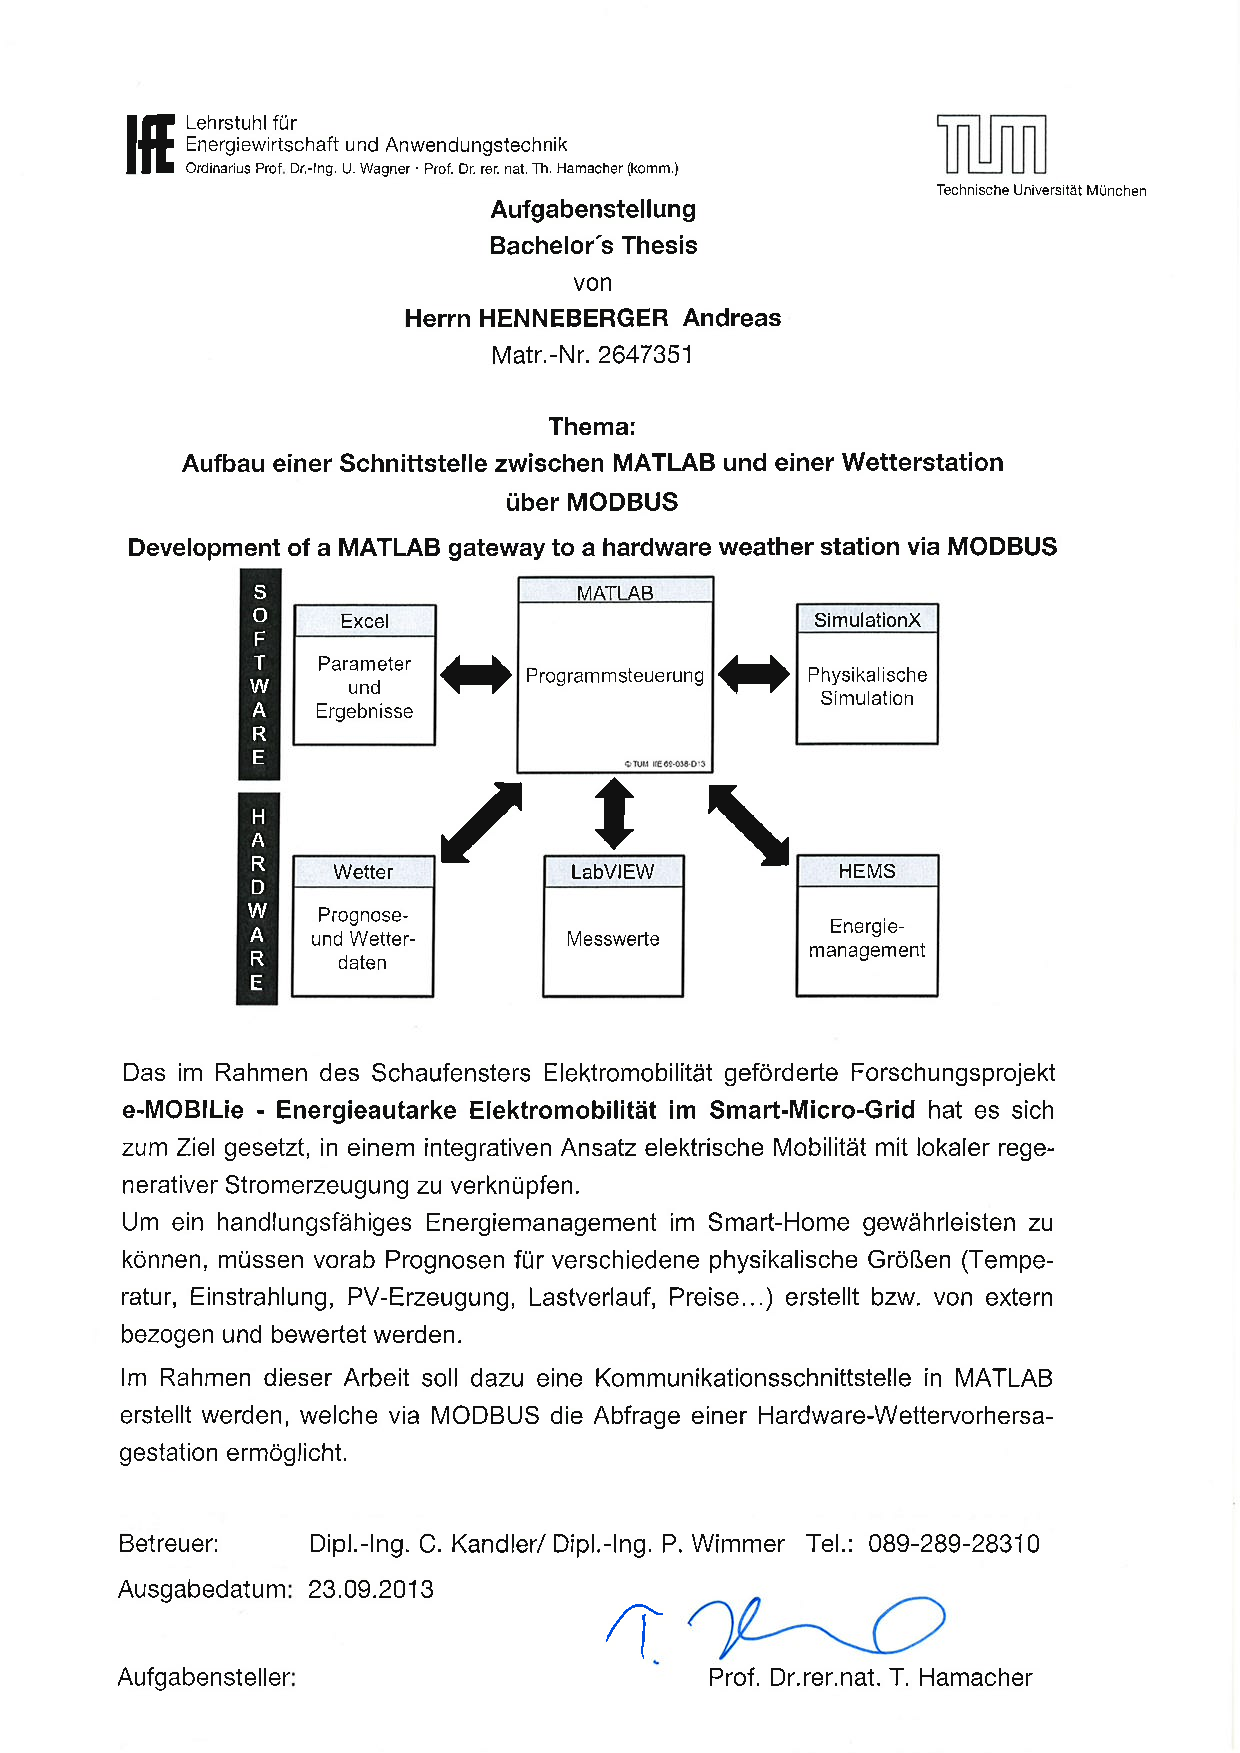
\includepdf[pages={1}]{task.pdf}
\noindent Hiermit erkläre ich,\\
Name: Henneberger\\
Vorname: Andreas Helmut\\
Mat.Nr.: 2647351\vspace{0.4cm}\\
dass ich die beiliegende Bachelor's Thesis zum Thema:\vspace{0.5cm}\\
\begin{center}
\textbf{Aufbau einer Schnittstelle zwischen Matlab und einer Wetterstation über MODBUS}
\end{center}\vspace{0.4cm}
selbständig verfasst, keine anderen als die angegebenen Quellen und Hilfsmittel benutzt habe,
sowie alle wörtlichen und sinngemäß übernommenen Stellen in der Arbeit gekennzeichnet und die 
entsprechenden Quellen angegeben habe.\\
Vom Lehrstuhl und seinen Mitarbeitern zur Verfügung gestellte Hilfsmittel, wie Modelle oder
Programme, sind ebenfalls angegeben. Diese Hilfsmittel sind Eigentum des Lehrstuhls bzw. des
jeweiligen Mitarbeiters. Ich werde sie nicht über die vorliegende Arbeit hinaus weiter verwenden
oder an Dritte weitergeben.\vspace{0.5cm}\\

\noindent Einer weiteren Nutzung dieser Arbeit und deren Ergebnisse (auch Programme und Methoden) zu Zwecken
der Forschung und Lehre, stimme ich zu.\vspace{0.5cm}\\

\noindent Ich habe diese Arbeit noch nicht zum Erwerb eines anderen Leistungsnachweises eingereicht.\vspace{0.5cm}\\

\noindent München, \date{\today}\vspace{0.5cm}\\
\noindent ...........................................\\
Andreas Henneberger
\tableofcontents
\listoffigures
\listoftables
\part{Einleitung}
Schenkt man der Studie von \enquote{Global EV Outlook} glauben, so wird die Mobilität in Zukunft durch elektrisch angetriebene Autos mit geprägt sein \cite{EVOutlook}. Damit Deutschland auf diesem Technologiefeld eine Spitzenposition einnehmen kann, wurde von der Bundesregierung die Nationale Plattform Elektromobilität initiiert. Ziel dieser Institution ist es Deutschland bis zum Jahr 2020 zum Leitmarkt und Leitanbieter zu entwickeln. Marktvorbereitung, Markthochlauf und der Massenmarkt sind dabei die zu durchlaufenden Phasen. In der Marktvorbereitungsphase, in der wir uns zur Zeit befinden, werden die Ergebnisse aus Forschung und Entwicklung genutzt, um in vier sogenannten Schaufenstern die Modelle und Prognosen für den Markthochlauf zu validieren bzw. bei auftretenden Abweichungen anzupassen \cite{NPE}. Eines dieser Schaufenster, genannt "{}Elektromobilität verbindet"{} wird von den Bundesländern Bayern und Sachsen betreut und finanziert. Das Schaufenster ist aufgegliedert in vier Teilprojekte von denen eines sich den Energiesystemen widmet. Das Themengebiet Energiesysteme ist wiederum in 9 Aufgabengebiete unterteilt, wovon sich eines mit der Integration der Elektromobilität in die dezentrale regenerative Energieversorung beschäftigt. Ein Aufgabenschwerpunkt hierbei ist es ein integriertes Energiemanagementsystem mittels Aufbau und Betrieb eines Hardware-in-the-Loop Prüfstands zu evaluieren \cite{SEEV}. Da es sich hierbei um ein Einfamilienhaus handelt spricht man von einem Home Energiemanagementsystem (HEMS). Was ist die Aufgabe eines solchen Systems und was macht ein solches System aus? Eine Antwort auf diese Fragen gibt der Artikel \enquote{Link to future} auf den sich die nachfolgenden Angaben beziehen \cite{LtoF}. Hier ist es Aufgabe eines HEMSs den Nutzer mit umfassenden Funktionen zum internen Informationsaustausch zu versorgen. Diese Informationen dienen letztendlich dazu den täglichen Energieverbrauch zu optimieren, um dadurch bei gleichbleibender Lebensqualität Kosten zu sparen. Drei Bausteine bilden dabei das Grundgerüst für das HEMS. 
\begin{enumerate}
\item Das \enquote{Energy Management Gateway} übernimmt dabei die Aufgabe des sicheren Datenaustauschs zwischen den hausinternen Gerätschaften sowie über das Versorgungsnetz zu den Energieversorgern. 
\item Die \enquote{Energy Management Unit (EMU)} sammelt alle Daten über den Energieverbrauch, die Energieerzeugung sowie -speicherung in einem Haushalt. Abgeleitet aus diesen Informationen und den momentanen Preisen für Energieverbrauch und -erzeugung regelt sie den Einsatz der Geräte. 
\item Die Bereitstellung von Informationen für die EMU erledigt ein Netzwerk von Sensoren und Microcontrollern. Hierzu wird häufig ein Home Area Network entweder drahtgebunden oder über Funk installiert.     
\end{enumerate} 
Diese Arbeit orientiert sich am dritten Baustein und soll Wetterdaten, einer später extern am Haus angebrachten Wetterstation, der EMU zur Verfügung stellen. Die EMU wird hierbei durch ein MATLAB-Programm dargestellt. 
\part{Hauptteil}
\chapter{Aufbau der Wetterstation}
\section{Aufbau der Datenstruktur}
An dieser Stelle der Bachelorarbeit sollen die grundlegenden Eigenschaften der verwendeten Wetterstation dargestellt werden. Eine gute Kenntnis der Datenstruktur sowie der Datenbereitstellung sind eine zwingende Voraussetzung für den späteren Aufbau der MATLAB Funktion. Der Hersteller bietet für die Hardware eine Reihe von Lizenzmodellen an, die den Empfang der Datenmenge bestimmt. Das in dieser Arbeit zum Einsatz kommende Modell nennt sich "{}WS-K RTU485 WPAia T"{} und beinhaltet das Prognosepaket "Premium All inclusive advanced", welches es ermöglicht, das komplette Spektrum an Prognosedaten abzurufen\cite[S. 2]{HKWDoc}. Welche Wetterinformationen genau zur Verfügung stehen, kann der unten aufgeführten Grafik entnommen werden.
\begin{figure}[h]
\centering
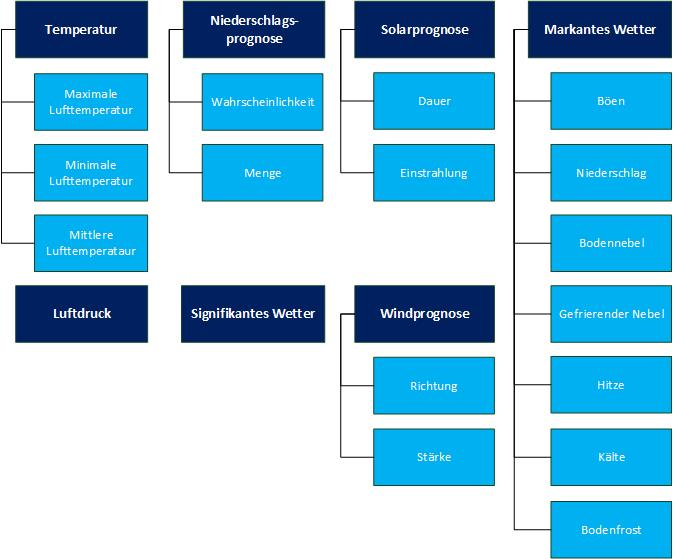
\includegraphics[scale=0.65]{weatherstation/Datenuebersicht}
\caption{Verfuegbare Prognosedaten WS-K RTU485 WPAia\cite[S. 5]{HKWDoc}}
\label{fig:1}
\end{figure}
Für welche Bereiche diese metereologischen Daten zutreffen muss in der Wetterregion spezifiziert werden. Hier besteht die Möglichkeit für über 1000 Städte in fast ganz Europa die Wetterprognosen abzufragen\cite[S. 27-38]{HKWDoc}. Wie schon in der Einleitung erwähnt, wäre eine niedrige zeitliche Auflösung der Daten wünschenswert, damit das Energiemanagementsystem ohne große Verwerfungen planen kann. Jedoch liegen die meisten Daten in einer Auflösung von 6 Stunden vor, d.h. für ein Intervall von morgens, mittags, nachmittags und abends. Lediglich die mittlere Lufttemperatur wird in einer 1 stündigen Auflösung bereitgestellt. Dieser Umstand wird später im Programmablauf gesondert berücksichtigt. Ein Update der Daten erfolgt ebenfalls alle 6 Stunden. Neben der Auflösung unterscheidet sich auch der Prognosehorizont innerhalb der zugänglichen Daten. Die Spanne reicht von einem bis zu drei Folgetagen. Für den aktuellen Tag, liegen für alle Bereiche Daten vor. Welche metereologische Ausprägung welche Eigenschaften besitzt, kann in der Tabelle\ref{fig:detaildatenstruktur} im Anhang nachvollzogen werden.    
\section{Technischer Aufbau der Station}
\subsection{Senderauswahl und Stationsaufbau}
Die eingesetzte Wetterstation erhält ihre Daten via Langwelle von drei auswählbaren Sendern:
\begin{itemize}
\item Sender Mainflingen DCF 49
\item Sender Burg DCF 39
\item Sender Lakihegy HGA 22 (Ungarn)
\end{itemize}
\begin{figure}[h]
\centering
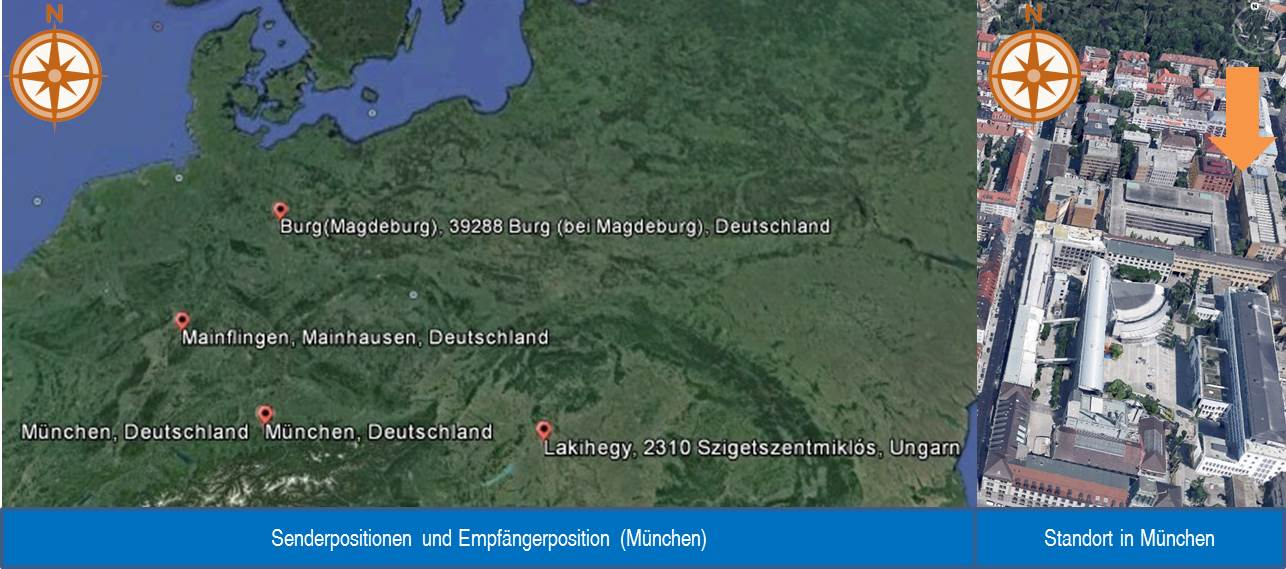
\includegraphics[scale=0.65]{weatherstation/Empfaengerausrichtung}
\caption{Standorte der Langwellensender und des Empfängers\cite[S. 15]{HKWDoc}}
\label{fig:3}
\end{figure}
Die Wetterstation soll in München aufgebaut werden. Um einen guten Empfang gewährleisten zu können, muss sie entsprechend ausgerichtet werden. Der Hersteller gibt hierzu Kriterien vor, die beachtet werden sollten\cite[S. 13 u. 15]{HKWDoc}:
\begin{itemize}
\item senkrechter Aufbau des Gehäuses mit nach unten austretendem Kabelstrang
\item für einen Innenaufbau in der Nähe zum Fenster
\item Mindestabstand von 30 cm zu Metallkonstruktionen oder -flächen
\item ausreichende Entfernung zu Geräten die elektromagnetisch abstrahlen
\item keine direkte Sonnenbestrahlung für das Einbinden der lokalen Temperatur
\item ausreichender Bodenabstand, um Einschneien zu vermeiden
\item Ausrichtung zum geografisch günstigsten Sender
\end{itemize} 
Unter Berücksichtigung dieser Empfehlungen wurde die Station in Fensternähe in nordwestlicher Richtung aufgebaut und die Sendestation Mainflingen vorgegeben.
\subsection{Registereinteilung und Schnittstellenparametrierung}
Wie im vorigen Kapitel bereits erläutert, können über das MODBUS Protokoll vier Arten von Registern angesprochen werden. In der Wetterstation sind zwei Register für die Kommunikation vorgesehen. Im Holdingregister können Einstellungsparameter gesetzt und gelesen werden. Eine Übersicht gibt die oben aufgeführte Tabelle \ref{tab:kommeinstpara}.
\begin{table}[t]
\rowcolors{1}{cyan}{white}
{
\setlength{\extrarowheight}{0.1cm}
\begin{tabular}{| c | l | c | l | l | p{2.5cm} |}
\hline
\textbf{\parbox[t]{2cm}{Register-\\adresse}} & \textbf{Bezug} & \textbf{Zugriff} & \textbf{Datentyp} & \textbf{Bereich} & \textbf{Bemerkung}\\[1cm]
\hline \hline
\hiderowcolors
110 & Senderstation & Lesen/Schreiben & unsigned & 0,1,2 & 0 = DCF 49 \newline 1 = HGA 22 \newline 2 = DCF 39\\
111 & Empfangsqualität & Lesen & unsigned & 0...9 & 9 ist höchste Qualität\\
112 & Stadt ID & Lesen/Schreiben & unsigned & 0...1022 & \\
100 & Sekunde (Funkuhr) & Lesen & unsigned & & UTC\\ 
101 & Minute (Funkuhr) & Lesen & unsigned & & UTC\\
102 & Stunde (Funkuhr) & Lesen & unsigned & & UTC\\
103 & Tag (Funkuhr) & Lesen & unsigned & & UTC\\
104 & Monat (Funkuhr) & Lesen & unsigned & & UTC\\
105 & Jahr (Funkuhr) & Lesen & unsigned & & UTC\\
\hline
\end{tabular}
}
\caption{Einstellungsparameter für den Kommunikationsaufbau und den Wetterbereich \cite[S. 16-17]{HKWDoc}}
\label{tab:kommeinstpara}
\end{table} 
Außerdem sind sämtliche metereologischen Daten in diesem Register abgelegt. Eine Auflistung der den Prognosebereichen zugeordneten Registeradressen gibt die im Anhang befindliche Tabelle\ref{fig:detaildatenstruktur}. Es ist dabei zu beachten, dass die Adressen gegenüber den in der Spezifikation des Herstellers Angegebenen, bereits auf die Struktur des Holdingregisters angepasst wurden. D.h. da das Holdingregister mit einer 0 beginnt, wurde von jeder Adresse eine Position abgezogen. Neben dem Holdingregister gibt es noch das Coilregister, in welchem die Zustände für den externen Temperatursensor und die FSK Qualität vorgehalten werden. Die Adressen hierfür sind 1 bzw. 2 und die zugelassenen Werte 1 und 0 geben jeweils den Zustand an. 1 bedeutet der Sensor sowie die FSK Qualität sind in Ordnung. 


    

\chapter{Das Modbus-Protokoll}
Nachdem die Wetterstation über MODBUS kommuniziert, soll in diesem Kapitel das MODBUS Protokoll näher erläutert werden. Dabei wird überwiegend Bezug auf die offizielle MODBUS Spezifikation genommen \cite{ModbusDoc}. Angesiedelt auf der ersten, zweiten und siebten Ebene des OSI Modells und damit einfach zu handhaben, ist MODBUS als Kommunikationsprotokoll in der Industrie weit verbreitet. Die unten stehende \textbf{Abbildung \ref{fig:prinzip}} dient zur ersten Orientierung der nachfolgend behandelten Themengebiete. 
\begin{figure}[hbtp]
\centering
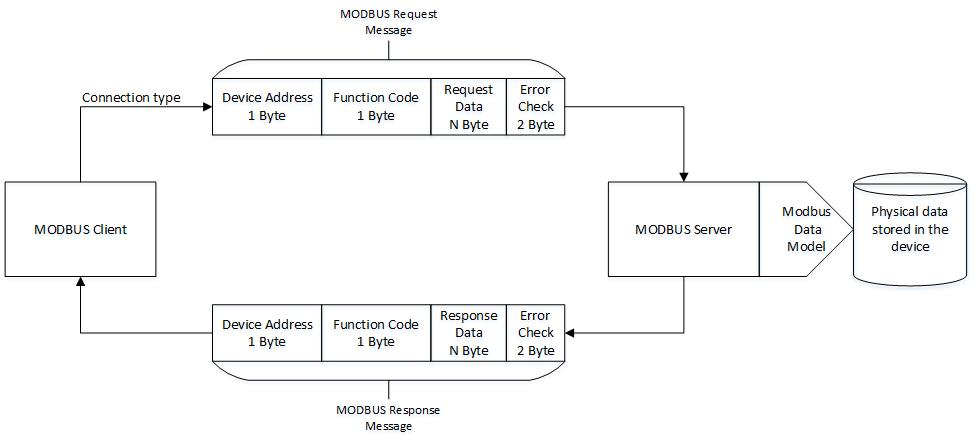
\includegraphics[scale=0.65]{modbus/msgskizze2}
\caption{Skizze der Funktionsweise des MODBUS Protokolls \cite[S. 5]{modicon}}
\label{fig:prinzip}
\end{figure}
\section{Verbindungstypen}
Es ist möglich das Protokoll auf drei Verbindungstypen zwischen Client und Server einzusetzen. Dazu zählen: 
\begin{itemize}
\item eine Internetverbindung TCP/IP 
\item eine asynchrone serielle Verbindung (z.B. RS-232, RS-422, RS-485, etc.)
\item eine MODBUS Plus Verbindung  
\end{itemize}
In dieser Arbeit ist die Wetterstation seriell über eine RS-485 Schnittstelle mit dem Rechner verbunden. 

Die RS-485 Schnittstelle bietet den Vorteil, dass die Verbindung der Netzwerkteilnehmer wie bei einer RS-232 Schnittstelle nur über eine Zweidrahtleitung erfolgen kann. Jedoch können im Gegensatz zur RS-232 Schnittstelle bis zu 32 Teilnehmer im Netzwerk angeschlossen werden. Die Netzwerklänge kann ohne Verstärker bis zu 1200 m betragen.\cite{Schleicher.2008} 

Diese Eigenschaften bieten sich an, um die Wetterstation wie in der Einleitung erwähnt, in ein Sensornetzwerk zu integrieren. Das Energiemanagementsystem kann die Daten entsprechend auslesen und Aktoren einstellen.
\section{Nachrichtenaufbau}
Wie eine typische MODBUS Nachricht aufgebaut ist, zeigt die unten stehende \textbf{Abbildung \ref{fig:modbusmessage}}. 
\begin{figure}[h]
\centering
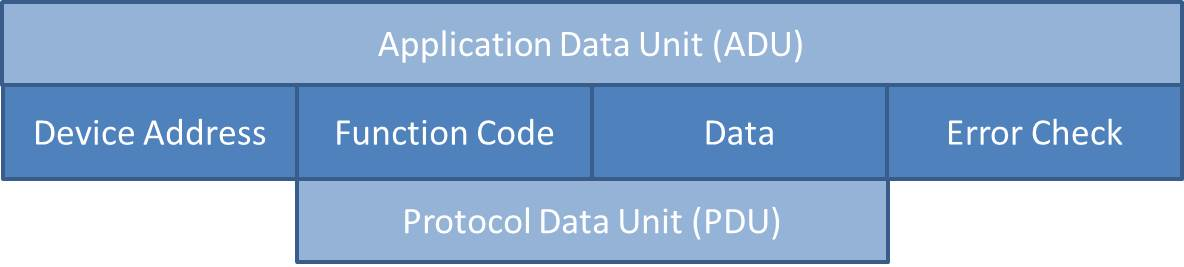
\includegraphics[scale=0.65]{modbus/ADUPDU}
\caption{Aufbau einer MODBUS Nachricht}
\label{fig:modbusmessage}
\end{figure} 
Die PDU ist unabhängig vom Netzwerk auf dem das Protokoll eingesetzt wird und setzt sich aus dem Funktionscode und den zu übermittelnden Daten zusammen. Mit einem Byte codiert gibt der Funktionscode an, ob eine schreibende oder lesende Kommunikation an welcher Art Register vorgenommen werden soll. Er kann aber auch einfach nur eine Aktion ausführen. In der Spezifikation werden drei Funktionscodearten genannt, öffentliche, benutzerdefinierte und reservierte Funktionscodes von denen in dieser Arbeit aber nur die Öffentlichen interessieren. Im Falle einer Anfrage des Client, enthält der Datenblock die entsprechenden Informationen über die genaue Adresse und Anzahl der zu lesenden oder beschreibenden Register. Für einen Schreibprozess wird hier auch der notwendige Input angegeben. Die abgefragten Daten des Servers sind ebenfalls im Datenblock untergebracht. Ein besonderes Augenmerk muss auf die Adressierung im Datenblock gelegt werden. Da hier nur die Startadresse angegeben wird und die Anzahl der nachfolgenden Adressen, ist es nicht möglich mit einer Nachricht nicht konsekutive Registeradressen auszulesen oder zu beschreiben. Hierfür wäre jeweils eine eigene Nachricht notwendig. Die Slave-ID und der Error-Check sind Informationen, die für das Netzwerk sprich den Verbindungstyp zwischen den Geräten eine Rolle spielen. Wie eben kurz skizziert, unterscheidet das MODBUS Protokoll zwischen drei Arten von PDUs, die nachfolgend zusammengefasst aufgeführt sind:
\begin{itemize}
\item die Anfrage-PDU besteht aus dem Funktionscode und den Anfragedaten
\item die Antwort-PDU besteht ebenfalls aus einem Funktionscode und den Antwortdaten
\item die Fehler-PDU besteht aus dem Fehlerfunktionscode (Funktionscode + 0x80 hex) und der Fehlermeldung 
\end{itemize}
Die Bytereihenfolge im Datenblock folgt der big-endian Anordnung, d.h. das Most Significant Bit kommt an erster und das Least Significant Bit an letzter Stelle. 
\section{Registertypen}
Die Daten, die vom Client abgefragt werden können, müssen physikalisch im Speicher des Servers liegen. Eine Verknüpfung dieses Speichers mit den zur Verfügung stehenden Registern im MODBUS Protokoll ermöglicht den Zugriff. Es werden vier Registerarten unterschieden, die in der \textbf{Tabelle \ref{tab:regartenmodbus}} aufgezeigt sind.
\begin{table}[htbp]
\caption{Übersicht der Registerarten im MODBUS Protokoll}
\rowcolors{1}{cyan}{white}
{
\setlength{\extrarowheight}{0.1cm}
\begin{tabular}{| l | l | l | p{6.5cm} |}
\hline
\textbf{Register} & \textbf{Wortlänge} & \textbf{Zugriff} & \textbf{Info}\\[0.5cm]
\hline \hline
\hiderowcolors
Diskreter Input & 1 Bit & Lesen & Daten werden durch ein I/O System bereitgestellt \\
Coils & 1 Bit & Lesen/Schreiben & Daten können über ein Anwendungsprogramm geändert werden \\
Input Register & 16 Bit & Lesen & Daten werden durch ein I/O System bereitgestellt \\
Holding Register & 16 Bit & Lesen/Schreiben & Daten können über ein Anwendungsprogramm geändert werden \\ 
\hline
\end{tabular}
}

\label{tab:regartenmodbus}
\end{table}
Jedes dieser Register besitzt einen Adressraum der bei 0 beginnt und bei 65535 endet. Zieht man noch eine weitere Quelle heran, so liegen die gültigen Adressbereiche jedoch anders verteilt vor. So besitzen die Coil-Register nur einen gültigen Adressraum von 1-9999, der Diskrete Input einen von 10001-19999, das Input Register einen von 30001-39999 und das Holding Register ab der Adresse 40001-49999 \cite{modicon}.    
\section{Nachrichtenverarbeitung}
Die \textbf{Abbildung \ref{fig:modbustransdiag}} im Anhang zeigt den Ablauf einer Nachrichtenüberprüfung und an welcher Position welcher Fehlercode gesendet wird, wenn die Nachricht fehlerhaft ist. Die Umsetzung dieser Überprüfung erfolgt später in der rx-Datenverarbeitung in Kapitel~\ref{sec:rxdatenverarbeitung} auf Seite~\pageref{sec:rxdatenverarbeitung}. 
\section{Funktions- und Fehlercodes}
Wie bereits erwähnt, ist der Funktionscode ein entscheidender Baustein in der MODBUS Nachricht. Es ist daher von Vorteil die für die Zwecke dieser Arbeit Wichtigen zu identifizieren, um das Handling des Programms zu vereinfachen. Die im Anhang dargestellte \textbf{Abbildung \ref{fig:fcodetab}} zeigt die zur Verfügung stehenden Funktionscodes. Gelb markiert sind dabei die Codes, die für die Kommunikation zwischen MATLAB und der Wetterstation Bedeutung haben. Bei dem Versuch diese Funktionscodes auszuführen, wurden lediglich Fehlercodes mit der Ausnahme 1 zurückgegeben. Daher ist davon auszugehen, dass die Funktionscodes für den Bereich Services File Record Access, Diagnostics und Other in dieser Hardware nicht gültig sind.    
Wie schon im Abschnitt~\ref{coilabfrage} auf Seite~\pageref{coilabfrage} beschrieben, müssen für den Fall einer Abfrage der Zustände des Temperatursensors oder der FSK Qualität die Coiladressen 0 oder 1 ausgelesen werden. Hierzu reicht es also jeweils eine Adresse in der MODBUS Nachricht anzugeben und die auszulesende Adresszahl auf 1 zu setzen. Die Anfrage- und Antwortnachricht für einen funktionierenden Temperatursensor ist in der \textbf{Tabelle \ref{tab:coilnachricht}} beispielhaft mit allgemeingültigen Ergänzungen dargestellt. Alle zwei Byte breiten Worte, wie zum Beispiel die Startadresse, setzen sich aus einem sogenannten High-Byte (H-Byte) und einem Low-Byte (L-Byte) zusammen.
\begin{table}[htbp]
\caption{Aufbau einer lesenden Kommunikation mit einem Coil-Register }
\rowcolors{1}{cyan}{white}
{
\setlength{\extrarowheight}{0.1cm}
\begin{tabular}{| l | l | l | p{7.5cm} |}
\hline
\textbf{\parbox[t]{2.6cm}{Nachrichten-\\typ}} & \textbf{\parbox[t]{2.6cm}{Nachrichten-\\teil}} & \textbf{\parbox[t]{1.7cm}{Wort-\\länge}} & \textbf{Inhalt}\\[0.25cm]
\hline \hline
\hiderowcolors
Anfrage & Funktionscode & 1 Byte  & 0x01 \\
 		& Startadresse  & 2 Bytes & H-Byte 0x00 L-Byte 0x00 (0x0000 bis 0xFFFF möglich) \\
        & Adressanzahl  & 2 Bytes & H-Byte 0x00 L-Byte 0x01 (1 bis 2000 (0x7D0) möglich) \\
Antwort & Funktionscode & 1 Byte  & 0x01 \\
		& Byteanzahl    & 1 Byte  & 0x01 (Ist das Ergebnis von Adressanzahl mod 8 = 0, so ergibt sich die Byteanzahl aus dem Ergebnis der Adressanzahl dividiert durch 8, andernfalls wird um ein Byte erhöht.)\\
		& Coil Status   & n Bytes & 0x01 (8 Coilzustände werden mit einem Byte, hier 00000001 angezeigt. Das Most Significant Bit im Antwort Byte steht dabei für die höchste Registeradresse.)\\ 
\hline
\end{tabular}
}
\label{tab:coilnachricht}
\end{table} 
\begin{table}[htbp]
\caption{Aufbau einer schreibenden Kommunikation mit einem Holding-Register }
\rowcolors{1}{cyan}{white}
{
\setlength{\extrarowheight}{0.1cm}
\begin{tabular}{| l | l | l | p{7.5cm} |}
\hline
\textbf{\parbox[t]{2.6cm}{Nachrichten-\\typ}} & \textbf{\parbox[t]{2.6cm}{Nachrichten-\\teil}} & \textbf{\parbox[t]{1.7cm}{Wort-\\länge}} & \textbf{Inhalt}\\[0.25cm]
\hline \hline
\hiderowcolors
Anfrage & Funktionscode    & 1 Byte  & 0x06\\
 		& Registeradresse  & 2 Bytes & H-Byte 0x00 L-Byte 0x70 (0x0000 bis 0xFFFF möglich)\\
        & Registerinput    & 2 Bytes & H-Byte 0x01 L-Byte 0x61 (0x0000 bis 0xFFFF möglich)\\
Antwort & Funktionscode    & 1 Byte  & 0x06\\
		& Registeradresse  & 2 Byte  & H-Byte 0x00 L-Byte 0x70\\
		& Registerinput    & 2 Byte  & H-Byte 0x01 L-Byte 0x61\\ 
\hline
\end{tabular}
}
\label{tab:writehreg}
\end{table}
\begin{table}[htbp]
\caption{Aufbau einer lesenden Kommunikation mit einem Holding-Register }
\rowcolors{1}{cyan}{white}
{
\setlength{\extrarowheight}{0.1cm}
\begin{tabular}{| l | l | l | p{7.2cm} |}
\hline
\textbf{\parbox[t]{2.6cm}{Nachrichten-\\typ}} & \textbf{\parbox[t]{2.6cm}{Nachrichten-\\teil}} & \textbf{\parbox[t]{1.7cm}{Wort-\\länge}} & \textbf{Inhalt}\\[0.25cm]
\hline \hline
\hiderowcolors
Anfrage & Funktionscode  & 1 Byte      & 0x03\\
 		& Startadresse   & 2 Bytes     & H-Byte 0x00 L-Byte 0x00 (0x0000 bis 0xFFFF möglich)\\
        & Adressanzahl   & 2 Bytes     & H-Byte 0x00 L-Byte 0x60 (1 bis 125 (0x7D) möglich)\\
Antwort & Funktionscode  & 1 Byte      & 0x03\\
		& Byteanzahl     & 2 Byte      & 2 x N (N = Adressanzahl)\\
		& Registeroutput & N x 2 Bytes & \\ 
\hline
\end{tabular}
}
\label{tab:readhreg}
\end{table}
Ein weiterer wichtiger Funktionscode ist der Code 0x06, mit dem man in das Holding-Register Werte schreiben kann. Wie im Abschnitt~\ref{comsetreg} auf Seite~\pageref{comsetreg} in der \textbf{Tabelle \ref{tab:kommeinstpara}} nachzulesen, wird die zu beobachtende Wetterregion mit einem Wert im Holdingregister an der Adresse 112 festgelegt. Für die Definition der Wetterregion München (Wert 353 dezimal) ist die hierzu notwendige Kommunikation in der \textbf{Tabelle \ref{tab:writehreg}} als Beispiel skizziert. Der wohl wichtigste und am meisten verwendete Funktionscode in dieser Arbeit ist der Code 0x03 zum Lesen des Holding-Registers. Über ihn werden sämtliche Prognosedaten ausgelesen. Auch hier soll ein Beispiel in der \textbf{Tabelle \ref{tab:readhreg}} den Aufbau verdeutlichen. In dem gezeigten Beispiel werden alle Wetterdaten, insgesamt 96 Werte, für die Mittlere Temperaturprognose abgerufen. 

Schlägt ein Kommunikationsprozess fehl, so wird vom Server statt der Antwortnachricht eine Fehlernachricht gesendet. Es sind folgende Fehlernachrichten vorgesehen:
\begin{itemize}
\item Code 01 Ungültige Funktion
\item Code 02 Ungültige Adressdaten
\item Code 03 Ungültige Daten
\item Code 04 Fehler beim MODBUS Server
\end{itemize}
Code 01 kann auftreten, wenn die entsprechende Funktion im Gerät nicht implementiert ist oder der Server sich in einem falschen Zustand befindet. Code 02 wird dann gesendet, wenn in der Anfrage mehr Register ausgelesen werden sollen, als zur Verfügung stehen. Code 03 gibt an, dass es sich bei dem im Datenblock befindlichen Wert um einen für den Server nicht Gültigen handelt. Code 04 wird übermittelt, wenn beim Server während der Bearbeitung der Anfrage ein Fehler aufgetreten ist.    
\section{Cyclic Redundancy Check}\label{chp:CRC}
Im MODBUS Protokoll sind zwei Modi definiert, wie die Nachrichten aufgebaut sein können. Da die Wetterstation aber im RTU Modus betrieben wird, muss der ASCII Modus in dieser Arbeit nicht berücksichtigt werden. Die Methode zum Absichern der Datenintegrität im RTU Modus ist der Cyclic Redundancy Check. Der Master sendet die MODBUS Nachricht an den Client, der wiederum den CRC Wert aus der Slave-ID, und der ADU berechnet. Kommt er auf ein anderes Ergebnis als es im CRC Wert steht, wird er die Anfrage nicht beantworten und es kommt zu einem Fehler, den der Master lösen muss.\cite{modicon} 

Analog dem Algorithmus aus dem Buch \enquote{Digitale Schnittstellen und Bussysteme} wird in MATLAB die CRC Prüfsumme berechnet. Zunächst wird die Nachricht aus Slave-ID und PDU (\textit{modbus\_pud\_hex}) an die Funktion \textsf{crc\_calc} übergeben. Die Länge dieser Nachricht geteilt durch zwei ergibt die enthaltene Anzahl an Bytes. Diese müssen im nächsten Schritt auf ein entsprechend breites binäres Bit Wort transformiert werden. Danach erfolgt die Initialisierung des Ausgangsschieberegisters, des Generatorpolynoms und der beiden Bytepositionszeiger \textit{m} und \textit{n}. Die MODBUS Nachricht wird durch die erste for-Schleife byteweise bearbeitet. Dabei werden die einzelnen Bytes zuerst auf 16 Bit breite Worte gebracht indem Nullen der rechten Seite zugewiesen werden. Danach folgt eine Exklusiv-Oder-Verknüpfung mit dem Ausgangsschieberegister 0xFFFF hex. Jetzt erfolgt für jedes Bit im aktuell anstehenden Byte ein Rechtsschieben bis das erste Bit mit einer eins herausgeschoben wurde. Die frei werdenden Bits auf der linken Seite werden mit Nullen aufgefüllt. Im nächsten Schritt wird mit dem Generatorpolynom wieder eine Exklusiv-Oder Operation durchgeführt und die Prozedur wird mit dem Ergebnis fortgesetzt. Am Ende wird das Resultat \textit{crc\_erg} dem Schieberegister zugewiesen und die Bytepositionszeiger erhöht. Sind alle Schleifen durchlaufen, wird zum Schluss das Schieberegister in einen 2 Byte hex Wert transformiert und mit der Slave-ID und der PDU zur ADU (\textit{txdata\_hex}) verknüpft.\cite{Schleicher.2008} 
\lstinputlisting[firstline=1, lastline=51]{modbus/crccalc.m}
\section{Simulation der Wetterstation}  
Nachdem nun die MODBUS und Wetterstationsspezifikation analysiert wurden, kann man mit der Umsetzung des MATLAB Programmes beginnen. Für den Fall, dass man noch nie in MATLAB mit einer seriellen Schnittstelle gearbeitet hat, bietet es sich an, diese zunächst einmal zu simulieren. Hierzu wurden in dieser Arbeit zwei Programme verwendet. Das eine Programm simuliert den COM Port des MODBUS Slave, heißt \enquote{Virtual Serial Ports Emulator} und wird von \enquote{eterlogic.com} zum Download angeboten \cite{eterlogic}. Das andere Programm virtualisiert den MODBUS Slave selbst und heißt \enquote{PeakHMI MODBUS Serial RTU slave}. Anbieter hierfür ist die Firma Everest Software LLC \cite{everest}. Der große Vorteil in der Simulation liegt darin, dass man in das virtualisierte Holdingregister an eine bestimmte Adresse Werte schreiben kann. Mit den Methoden von MATLAB kann man nun versuchen diesen Wert auszulesen. Mit dieser Methodik kann man schnell die Funktionalität des erarbeiteten Codes auch offline erproben. 

     
      

\chapter{Aufbau und Dokumentation des Programmcodes in MATLAB}
\section{Geforderte Funktionseigenschaften}
Die zu schreibende MATLAB Funktion soll nach Fertigstellung in weiteren MATLAB Programmen zum Einsatz kommen. Daher ist es wichtig, dass sämtliche Daten die für das Ausführen erforderlich sind bereits im Code vorliegen und nicht importiert werden müssen. Es sollen auch sonst nach dem Ausführen keine weiteren Maßnahmen oder Eingaben getätigt werden müssen. Um diese Voraussetzungen zu erfüllen müssen vor allem große Datensätze im Code eingebunden werden.\label{createstruct} Bei dieser Arbeit ist das zum einen die Städteliste mit ihren über 1000 Einträgen und zum anderen das Verzeichnis mit allen Registeradressen, in Summe über 340 Positionen. Daneben gibt es noch ein paar weitere Eigenschaften, die an dieser Stelle kurz aufgeführt werden.
\begin{itemize}
\item wiederholte Ausführung des Datenabrufs in bestimmten Zeitabschnitten ohne dabei MATLAB komplett zu blockieren
\item Handhabung der kompletten MODBUS Kommunikation, insbesondere des Datenabrufs, der -verarbeitung und der Parametersetzung
\item Interpolation der ausgelesenen Werte, um unterschiedliche zeitliche Auflösungen zu erhalten
\item Datensicherung derart, dass jeder Datenabruf in einer eigenen Datei und die Summe aller abgerufenen Werte in einer anderen Datei gespeichert werden
\item Fehlervermeidung bei der Eingabe von Inputparametern
\item Aufbau und Beendigung der seriellen Schnittstelle mit der Wetterstation
\item einfache und kurze Inputparameter
\end{itemize}
Nachdem die Eigenschaften nun bekannt sind, soll in den nachfolgenden Unterkapiteln die genaue Umsetzung im Programmcode erläutert werden. Hierzu wird zunächst eine grobe Struktur des Programmaufbaus in Abbildung \textbf{\ref{fig:flowchart}} gegeben. 
\begin{figure}
\centering
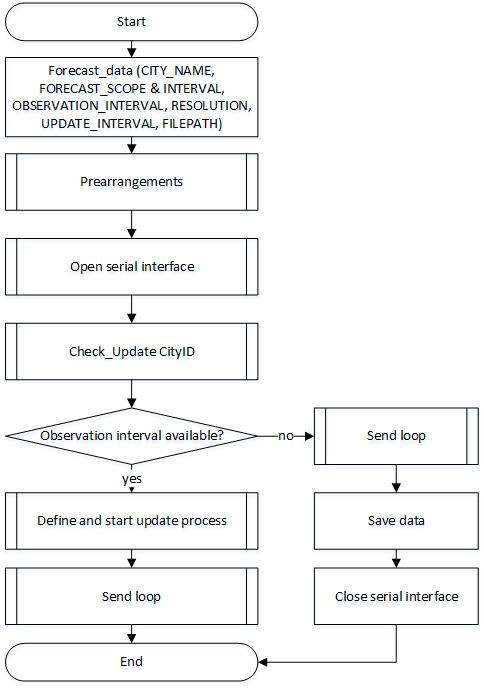
\includegraphics[scale=1]{programm/flowchart}
\caption{Ablaufplan der Funktion forecast\_data}
\label{fig:flowchart}
\end{figure} 
Wie in der Abbildung zu erkennen, ist es möglich für die Funktion forecast\_data sieben Eingabeparameter zu definieren. 
\begin{enumerate}
\item Wetterregion
\item Prognosebereichsdefinition
\item Start des Beobachtungszeitraums
\item Ende des Beobachtungszeitraums
\item zeitliche Auflösung
\item Updateintervall
\item Pfadangabe des Speicherortes (optional)
\end{enumerate}
Die Wetterregion wird als Stadtname in Stringformat übergeben. Die Prognosebereichsdefinition besteht aus drei Teilen, die als String in dieser Format 'Prognosebereich-Prognosedetail-Prognoseintervall' aufgebaut ist. Der erste Teil gibt den Wetterbereich an. Hier stehen alle Einträge in der Spalte Prognosebereich der Tabelle \ref{tab:detaildatenstruktur} im Anhang zur Verfügung. Die Prognosedetaildaten können der zweiten Spalte dieser Tabelle entnommen werden. Der dritte Parameter gibt die Anzahl der auszuwertenden Tage an, dabei steht der Wert 1 für den aktuellen Tag ohne Prognose und die Werte 2, 3, 4 für eine entsprechende Erweiterung des aktuellen Tages um die Prognosetage 1, 2 und 3 sofern vorhanden. Möchte man keine gesonderte Auswahl treffen und einfach alle möglichen Daten abrufen, so kann hier an dieser Stelle der Input 'all' erfolgen. Der Beobachtungszeitraum wird durch zwei Daten begrenzt, die ebenfalls als String in dieser Formation 'dd-mmm-yyyy', wobei mit mmm der englische Monatsname gemeint ist, angegeben werden. Die zeitliche Auflösung wird als Double eingetragen. Hier sind die Werte 1, 0.5, 0.25, 0.08 stellvertretend stehend für 1 Stunde, eine halbe Stunde, eine viertel Stunde und 5 Min., möglich. Ebenso als Double wir das Updateintervall definiert. Hier stehen die Werte 6, 12, 24 zur Verfügung, welches einem vier-, zwei- und einmaligen Update am Tag entspricht. Die Pfadangabe wird wiederum als String eingegeben. Die nächste Abbildung gibt hierzu ein Beispiel. Es wird für die Region München die Niederschlagsmenge für den heutigen und ersten Folgetag, die minimale Temperatur für den heutigen und die beiden nachfolgenden Tage, über einen Zeitraum von zwei Tagen abgerufen. Dabei beträgt die zeitliche Auflösung 1 Stunde und das Intervall in denen Updates gestartet werden 6 Stunden. Nachdem hier kein Speicherpfad angegeben ist, wird ein Ordner mit der Bezeichnung \enquote{Aufzeichnungen} im aktuellen MATLAB Ordner erstellt und als Speicherort ausgewählt. 
\begin{figure}
\centering
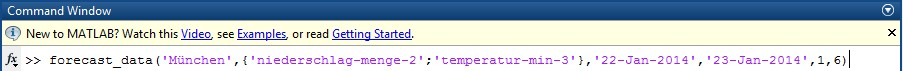
\includegraphics[scale=0.7]{programm/funkaufruf}
\caption{Beispiel für den Funktionsaufruf}
\label{fig:funkaufruf}
\end{figure} 
\section{Vorbereitende Maßnahmen}
\subsection{Zuweisung variabler Inputparameter und Variableninitiierung}
\lstinputlisting[firstline=69, lastline=124]{programm/forecastdata.m}
Für den Fall, dass variable Inputparameter übergeben wurden, wird zuerst geprüft, ob die Anzahl der geforderten Werte vorhanden ist. Ist das nicht der Fall, so wird eine Meldung an den Nutzer ausgeben und die Funktion beendet. Stimmt die Anzahl, werden die Werte Funktionsvariablen zugeordent. Ist zudem noch eine Pfadangabe zu einem Speicherort der Funktion übergeben worden, so wird diese ebenfalls einer Funktionsvariablen zugewiesen. Wurde keine Angabe hierzu gemacht, so wird im aktuellen MATLAB Ordner ein Ordner \enquote{Aufzeichnungen} als Speicherplatz definiert. Dabei wird nachgesehen, ob lediglich eine Laufwerksangabe vorliegt oder nicht. Existiert der Ordner bereits, erfolgt eine Meldung auf deutsch. Wurden keine variablen Parameter übergeben, so wird die zeitliche Auflösung auf 1 Stunde festgesetzt und ebenfalls ein Speicherort vorgegeben. Nachdem die \textit{forecast\_defintion} sowohl als String als auch als Cell-Array übergeben wird, im späteren Programmablauf aber nur ein Cell-Array erwartet wird, muss noch eine Konvertierung stattfinden.\label{sendloop}Mit dem ersten Funktionsaufruf, an dem noch kein Tageswechsel auftreten kann, werden die Variablen \textit{daychange\_flag} und \textit{daychange\_counter} auf Null gesetzt und dem Base-Workspace zugewiesen. Ebenso initialisiert werden die späteren Datencontainer \textit{weather\_data} und \textit{new\_data}. Wie in Tabelle \ref{tab:parabel} gezeigt, lautet die Slave-ID der Wetterstation \enquote{03}. Diese wird hier der \textit{device\_id} zugeordnet.    
\subsection{Aufbau von Strukturen}
\lstinputlisting[firstline=128, lastline=141]{programm/forecastdata.m} 
Wie bereits im vorigen Kapitel~\ref{createstruct} angekündigt, müssen große Datensätze in Strukturen gepackt werden um später aus ihnen Daten zu gewinnen. Sollen alle Wetterdaten abgerufen werden, ist es erforderlich ein Cell-Array aufzubauen, welches alle Wetterdatenanfragen beinhaltet. Danach werden Strukturen angelegt, die die Registeradressen und Städtenamen abbilden. Die letzten beiden Strukturen müssen wieder im Base-Workspace verfügbar sein da andere Funktionen auf sie zurückgreifen werden.
\subsection{Überprüfung der Eingabeparameter}
\lstinputlisting[firstline=145, lastline=169]{programm/forecastdata.m}
Diese for-Schleife bearbeitet alle übergebenen Wetterdatenanfragen, prüft sie auf Gültigkeit und erstellt zugleich die entsprechenden Datencontainer. Die Datencontainer werden im Base-Workspace eingetragen. Sind ein oder mehrere Eingabeparameter falsch, werden diese dem Nutzer mit einer Nachricht angezeigt und die Funktion beendet.
\lstinputlisting[firstline=1, lastline=1]{programm/inputcheck.m}
Die Funktion \textsf{input\_check} liefert als Outputparameter einen Vektor der angibt, welche Parameter gültig sind. Zusätzlich werden die generierten Fehlermeldungen, die ID der Wetterregion, der Breitengrad und Längengrad ausgegeben. 
\lstinputlisting[firstline=4, lastline=16]{programm/inputcheck.m}
Im ersten Abschnitt des Input Checks wird die Funktion \textsf{get\_city\_id} aufgerufen, um die ID der Wetterregion, den Längen- und Breitengrad zu ermitteln. Ist die ID nicht in der Liste zu finden, wird die entsprechende Vektorposition \textit{val\_inpt} auf false gesetzt.  
\lstinputlisting[firstline=1, lastline=18]{programm/getcityid.m}
In dieser Funktion muss zuerst die im Base-Workspace befindliche Variable \textit{city\_list} zugänglich gemacht werden. Danach wird die Spalte mit den Städtenamen mit \textsf{nominal} konvertiert, um im darauffolgenden Schritt eine einfache Suche der Position in der Liste zu starten, die dem Städtenamen entspricht. In der Variable \textit{city\_data\_set} sind nun alle Werte dieser Liste, die der Position entsprechen, enthalten. Eine einfache Wenn-Dann-Bedingung weist die Daten den Outputparametern zu.   
\lstinputlisting[firstline=19, lastline=62]{programm/inputcheck.m}
An dieser Stelle wird die Wetterdatenanfrage analysiert. Kommt in dem Ausdruck nicht zweimal ein Querstrich vor, ist die Eingabe schon fehlerhaft. Wenn doch, werden die drei einzelnen Bestandteile mit Listen abgeglichen und bei entsprechender Existenz keine Fehlermeldung ausgegeben.  
\lstinputlisting[firstline=65, lastline=103]{programm/inputcheck.m}
Die Überprüfung des Observationszeitraums erfolgt dahingehen, dass der Ausdruck ein Datumsformat darstellen muss, den MATLAB mittels \textsf{datenum} konvertieren kann. Ist dies nicht möglich, liegt ein Fehler vor. Sind die Datumsformate korrekt, so kann es immer noch der Fall sein, dass das Startdatum in der Vergangenheit oder vor dem Enddatum liegt. Auch hier werden entsprechende Fehlermeldungen generiert.
\lstinputlisting[firstline=105, lastline=132]{programm/inputcheck.m}
Im letzten Teil der Überprüfung werden die Werte der zeitlichen Auflösung und des Updateintervalls wieder mit Listen abgeglichen. Ist der Gültigkeitsvektor in der boolschen Überprüfung wahr, werden keine Fehlermeldungen ausgegeben. Andernfalls wenn weniger als 10 Fehlermeldungen angefallen sind, muss der letzte Vektoreintrag der Fehlermeldungen leer sein. Dies ist erforderlich, um den nachfolgenden Print-Befehl ausführen zu können. 
\subsection{Verfügbarkeitsprüfung der seriellen Schnittstelle}   
\lstinputlisting[firstline=173, lastline=189]{programm/forecastdata.m} 
Existiert bereits eine Variable \textit{serial\_interface} im Base-Workspace, so wird diese gelöscht. Zudem werden alle anderen seriellen Schnittstellen gelöscht um zu vermeiden, dass bereits eine andere serielle Schnittstelle den COM6 Port belegt hat. Danach wird die Verfügbarkeit des COM6 Ports festgestellt. Ist dies nicht der Fall, wird eine Fehlermeldung an den Nutzer ausgegeben und die Funktion beendet.
\section{Aufbau der seriellen Schnittstelle}
\lstinputlisting[firstline=191, lastline=192]{programm/forecastdata.m}
Die Funktion \textsf{open\_serial\_port} enthält bereits alle in der Tabelle \ref{tab:parabel} auf Seite~\pageref{coilabfrage} festgelegten Schnittstellenparameter.
\lstinputlisting[firstline=1, lastline=17]{programm/openserialport.m}
MATLAB bietet für den Aufbau einer seriellen Schnittstelle eine Funktion namens \textsf{serial} an. Diese wird hier zur Erstellung der Variable \textit{serial\_interface} angewandt. Die Variable wird dem Base-Workspace zugewiesen und die serielle Schnittstelle mit dem Befehl \textsf{fopen} geöffnet. Der Nutzer wird über den Schnittstellenaufbau informiert.
\section{Abgleich der Wetterregion im Register}
\lstinputlisting[firstline=195, lastline=221]{programm/forecastdata.m}
Da der Wechsel einer Wetterregion unter Umständen bis zu drei Tagen dauern kann, bis alle anliegenden Werte Gültigkeit besitzen, wird in diesem Teil des Codes zuerst die bereits eingetragene Stadt-ID ausgelesen und mit der in dem Funktionsaufruf Angegebenen verglichen. Weichen die beiden Werte voneinander ab, so wird der Nutzer per Tastatureingabe aufgefordert dem Wetterregionenwechsel zuzustimmen. Er hat somit die Gelegenheit einen versehentlichen Wechsel abzubrechen. Anschließend wird der neue Wert im Register eingetragen. 
\section{Festlegung der Timerparameter und Starten des Timers}
\lstinputlisting[firstline=226, lastline=263]{programm/forecastdata.m}
Um die Eigenschaft des wiederholten Datenabrufs zu implementieren wurde das Timer-Objekt von MATLAB implementiert. Es bietet den Vorteil im Hintergrund zu laufen ohne dabei MATLAB komplett zu blockieren. Für die Initialisierung dieses Objekts müssen zuerst ein paar Parameter ermittelt werden. Insbesondere betrifft dies das Timerintervall, die Anzahl der Timerausführungen und die Timerverzögerung. Das Timerintervall lässt sich einfach dadurch berechnen indem die Variable \textit{update\_interval} mit der Anzahl an Sekunden für eine Stunde multipliziert wird. Die Anzahl der Timerausführungen ergibt sich dann durch die zur Verfügung stehenden Stunden im Beobachtungszeitraum dividiert durch die Länge des Timerintervalls. Liegt der Beobachtungszeitraum in der Zukunft, so muss die Timerverzögerung genau die Länge vom Funktionsaufruf bis zum Startdatum aufweisen. Bei der Berechnung dieser Angaben sind die MATLAB Funktionen \textsf{days365}, \textsf{datevec} sowie \textsf{etime} äußerst nützlich.
\lstinputlisting[firstline=270, lastline=282]{programm/forecastdata.m}    
Mit der Zuweisung \enquote{t = timer} wird in der Variablen \textit{t} das Timer-Objekt erzeugt. Die Eigenschaften können dann ähnlich einer Struktur in MATLAB aufgerufen und bestimmt werden. Zu bestimmen sind die Timerverzögerung (\textit{t.StartDelay}), das Timerintervall (\textit{t.Period}), die Timerausführungen (\textit{t.TasksToExecute}), sowie die Ausführungsmethode (\textit{t.ExecutionMode}). Die Ausführungsmethode \enquote{fixedRate} garantiert, dass in genau gleichen Timerintervallen die in der Timerfunktion (\textit{t.TimerFcn}) definierte Funktion ausgeführt wird. Wird der Timer durch einen Fehler oder durch einen Abbruchbefehl unterbrochen, so legt man in der Timerstopfunktion fest, was geschehen soll.
\lstinputlisting[firstline=1, lastline=19]{programm/stoptimer.m}  
Kommt es zu einem Timerabbruch, so wird eine Meldung an den Nutzer ausgegeben, das Timer-Objekt gelöscht und der Datencontainer mit den fortlaufenden Werten abgespeichert. Außerdem wird die serielle Schnittstelle beendet. Der Dateiname für den Datencontainer setzt sich zusammen aus der Wetterregion, der angewandten zeitlichen Auflösung, dem aktuellen Datum und dem aktuellen Datum in Unix Zeitformat.    
\section{Abschicken der MODBUS-Anfragen}
\lstinputlisting[firstline=1, lastline=2]{programm/sendloop.m}
Die Funktion, die das sequentielle Abschicken und Verarbeiten der einzelnen MODBUS Nachrichten übernimmt wird hier erläutert.
\lstinputlisting[firstline=5, lastline=35]{programm/sendloop.m}
Nachdem die Eingabeparameter übergeben wurden, werden die im Base-Workspace vorhandenen Variablen \textit{daychange\_flag}, \textit{daychange\_counter}  sowie der Datencontainer \textit{w\_dat} für die Langzeitarchivierung in dieser Funktion bereitgestellt. Eine for-Schleife durchläuft dann alle Wetterdatenanfragen die in \textit{fc\_def} definiert wurden. Beim ersten Durchlauf muss geprüft werden, ob bereits zu einem früheren Zeitpunkt Daten ausgelesen wurden damit ein Tageswechsel signalisiert werden kann. Hierzu wird der letzte Zeitstempel des letzten Datenabrufs, sofern vorhanden, mit dem aktuellen Datum verglichen. Ist das Ergebnis ungleich Null, liegt ein Tageswechsel vor und die Variablen werden entsprechend angepasst und im Base-Workspace aktualisiert.
\lstinputlisting[firstline=38, lastline=94]{programm/sendloop.m}
Im nächsten Schritt wird das Intervall für die auszulesenden Wetterdaten zusammengestellt. Hierbei muss unterschieden werden zwischen den stündlichen Werten der mittleren Lufttemperatur, dem begrenzten Prognosehorizont von Luftdruck und Solarleistung und den verbleibenden Daten. Gibt der Nutzer eine zu hohe Zahl für Luftdruck oder Solarleistung ein, so wird auf die möglichen Werte angepasst und eine Warnung ausgegeben.
\lstinputlisting[firstline=95, lastline=111]{programm/sendloop.m}
In diesem Abschnitt wird die MODBUS Nachricht erstellt und einer Funktion übergeben, die das Schreiben und Lesen auf der seriellen Schnittstelle übernimmt. Die Startadresse des Registers ergibt sich aus dem Prognosebereich, dem Prognosedetail und dem Anfangszeitpunkt zu dem die Werte ausgelesen werden sollen. Die Endadresse wir im gleichen Verfahren ermittelt. Die Differenz aus den beiden Adressdaten ergibt die Registeranzahl. Gemäß der MODBUS Spezifikation liegen nun alle Daten vor, die zur Kommunikation notwendig sind. Lediglich der Cyclic Redundancy Check fehlt noch. Dieser wird in der Funktion \textsf{gen\_msg} erstellt und der PDU zusammen mit der Slave-ID angeheftet. Wie die momentane Verbindungsqualität zum Zeitpunkt der Anfrage ist, wird kurz darauf abgerufen. Alle für die weitere Verarbeitung erforderlichen Daten werden nun an die Funktion \textsf{send\_and\_receive\_data} übergeben. 
\lstinputlisting[firstline=112, lastline=131]{programm/sendloop.m}
Ist die for-Schleife durchlaufen und alle Daten liegen in den Datencontainern, wird der vollzogene Abruf in dem Container \textit{new\_data} mit entsprechendem Dateinamen abgespeichert. Der Dateiname setzt sich dabei aus dem Pfad zum Speicherort, dem Stadtnamen, der gewünschten Auflösung, dem aktuellen Datum und einem Datum in Unix Zeitformat zusammen. Ist das Speichern abgeschlossen, wird der Datencontainer geleert und neu initialisiert. Der letzte Schritt in diesem Programmteil ist das Update der noch verbleibenden Anzahl an Datenabrufen, welche in der Variable \textit{u\_c\_n} (update cycle number) hinterlegt sind.
\section{Senden und Empfangen}
\lstinputlisting[firstline=1, lastline=31]{programm/sendandreceivedata.m}
In dem Funktionsworkspace der Funktion \textsf{send\_and\_receive\_data} muss die serielle Schnittstelle zugänglich sein. Um die in der Funktion \textsf{send\_loop} generierte Nachricht über die Schnittstelle abschicken zu können, muss sie auf ein geeignetes Format gebracht werden. Dann erst kann die Nachricht mit dem Befehl \textit{fwrite} übermittelt werden. Es wird 1 Sekunde auf die Antwort gewartet. Das bestimmen der empfangenen Bytes und die Angabe beim Lesebefehl \textsf{fread} beschleunigt die Kommunikation enorm. Jetzt liegt die Antwortnachricht des Servers in der Variablen \textit{rx\_data} vor. Die darin enthaltenen Werte wurden als unsigned integer 8 bit empfangen.      
\lstinputlisting[firstline=1, lastline=31]{programm/formatmodbusmsg.m}
Die Funktion \textsf{format\_modbus\_msg} transformiert den String der MODBUS-Nachricht in einen 8-zeiligen Vektor mit dezimalen Werten die den hexadezimalen Werten des Strings entsprechen. 
\section{Rx-Datenverarbeitung}
\lstinputlisting[firstline=1, lastline=7]{programm/rxdataprocessing.m}
Hauptaufgabe der Rx-Datenverarbeitung ist es den empfangenen Funktionscode auszuwerten, die Daten zu isolieren und an eine weitere Funktion zur Bearbeitung zu übergeben. Der rx-Datenstring ist als Zeilenvektor aus einer Reihe von Dezimalzahlen folgendermaßen aufgebaut:
\begin{itemize}
\item an erster Stelle kommt die Slave-ID 
\item an zweiter Stelle folgt der Funktionscode 
\item an dritter Stelle steht die Anzahl der übertragenen Bytes
\item an den darauffolgenden Positionen befinden sich die Datenbytes
\item die beiden letzten Einträge beinhalten den CRC-Wert
\end{itemize}
\lstinputlisting[firstline=9, lastline=36]{programm/rxdataprocessing.m}
Zuerst wird der Funktionscode auf einen Fehlercode hin in der Funktion \textsf{fcod\_check} kontrolliert. Dies ist dann der Fall, wenn er nicht den Wert 1, 3 oder 6 besitzt. Um welchen Ausnahmefall es sich dann handelt, wird in der Switch-Abfrage geklärt und das Programm stoppt mit einem Fehler.  
\lstinputlisting[firstline=1, lastline=15]{programm/fcodecheck.m}
Ist der Funktionscode in Ordnung wird entschieden, wie mit den Datenbytes zu verfahren ist. Eine Switch-Abfrage führt zu den entsprechenden Arbeitsschritten. Für den Fall, dass der Funktionscode den Wert 1 oder 6 aufweist, ist die Bearbeitung recht einfach. Es müssen lediglich ein Datenbyte beim Code 1 und zwei Datenbytes beim Code 6 verarbeitet werden.    
\lstinputlisting[firstline=39, lastline=66]{programm/rxdataprocessing.m}

\section{Datenverarbeitung}
\lstinputlisting[firstline=1, lastline=1]{programm/dataprocessing.m}
Das eigentliche Herzstück dieses Programms ist die Datenverarbeitung die mit der Funktion \textsf{data\_processing} gestartet wird. Die notwendigen Parameter sind die empfangen Datenbytes im \textit{data\_string} hinterlegt, die Definition der Wetterdatenabfrage als \textit{fc\_def}, die zeitliche Auflösung in der Variable \textit{res}, die Verbindungsqualität, übergeben als \textit{con\_qual} und die Längen- und Breitengradangabe in Form von \textit{lng} bzw. \textit{lat}. 
\lstinputlisting[firstline=7, lastline=35]{programm/dataprocessing.m}
Zunächst werden die Variablen aus dem Base-Workspace geladen, mit denen gearbeitet wird. Danach liefert die Funktion \textsf{MESZ\_calc} ein Flag für die Mitteleuropäische Sommerzeit. Im Anschluß werden die Listen für einen späteren Datenabgleich erstellt.        
\lstinputlisting[firstline=37, lastline=47]{programm/dataprocessing.m}
Erfolgt nur eine Abfrage der Kommunikationsparameter oder bestimmter Zustände der Wetterstation, muss nur ein Wert ausgewertet werden. Dies geschieht, wenn die If-Bedingung wahr ist. Da die Daten der seriellen Schnittstelle als unsigned int8 Werte empfangen wurden, werden negative Werte ab der Zahl 32769 dargestellt. Um sie zu erhalten muss der Wertebereich von 2 unsigned Bytes abgezogen werden.  
\lstinputlisting[firstline=49, lastline=80]{programm/dataprocessing.m}
Ist die If-Bedingung falsch, handelt es sich um Wetterdaten. Zunächst werden Variablen initiiert. Dabei ist \textit{i} eine Laufvariable, die die Position angibt zu dem ein Datumswechsel stattgefunden hat. \textit{n\_dat\_r} ist die Vektorposition in dem Datencontainer, der jeden einzelnen Datenabruf speichert. Deshalb ist sie immer auf 1 gesetzt. Da die Ausgangsdaten selbst in einer unterschiedlichen Auflösung gegeben sind, müssen mit der Funktion \textsf{res\_factor} auch zwei separate Faktoren für die spätere Interpolation bestimmt werden. Hat ein Abruf bereit zu einem früheren Zeitpunkt stattgefunden, so wird dieser Abruf-Zeitstempel der Variable \textit{t\_rec} zugewiesen. Er bestimmt sich aus dem letzten aufgezeichneten Wert und dessen Rekordstempel. Anschließend wird die Startvariable \textit{sdindex} der nachfolgenden for-Schleife für die zu bearbeitenden Prognosetage bestimmt. Dabei definiert die Position in der entsprechenden Liste diesen Wert. Der Endwert \textit{edindex} der Schleife wird in gleicher Weise bestimmt.   
\lstinputlisting[firstline=82, lastline=118]{programm/dataprocessing.m}
Lag noch kein vorheriger Datenabruf vor, so starten die Positionsvektoren des Datencontainers, der die Daten des Beobachtungszeitraums speichert, bei 1. Hier werden zwei Variablen \textit{w\_dat\_r} und \textit{w\_dat\_org} benötigt. Während die Erste später mit der interpolierten zeitlichen Auflösung voranschreitet, behält die Zweite die ursprüngliche Schrittweite. Die while-Schleife bestimmt nun die Position bei einem evtl. Datumswechsel. Dazu wird die in der Variable \textit{unix\_t\_strt} gespeicherte Zeitreihe durchlaufen bis das Datum dem aktuellen Datum entspricht. Der Wert wird der Vektorposition übergeben. Abhängig ob es sich um Daten handelt die interpoliert werden, bekommt auch die Vektorposition für die originalen Daten einen Wert zugewiesen. Er errechnet sich entsprechend der Auflösung der Daten für die mittlere Lufttemperatur (24 Werte pro Tag) multipliziert mit der Zahl der bis dato vollzogenen Tageswechseln plus eins.      
\lstinputlisting[firstline=120, lastline=184]{programm/dataprocessing.m}
Handelt es sich um einen längeren Datenstring, so muss dieser durchlaufen werden. Es erfolgt eine Initialisierung dieser Variablen. Danach beginnt die Schleife für den Tagesdurchlauf. Zu Beginn wird je nach Schleifenpostition der Anfangs- und Endwert der Schleife für die Tagessegmente bestimmt. Der hier verwendete Aufbau scheint ein wenig kompliziert zu sein und stammt aus einer Version in der es möglich war völlig willkürliche Intervalle zu bestimmen und nicht nur tagesweise den Abruf zu durchlaufen. Sind Start- und Endwerte für die Tagessegment-Schleife bestimmt, wird im letzten Schritt das Datum der Schleifenposition ermittelt und in der Variablen \textit{date\_part} gespeichert. Diese wird später für die Berechnung der Unix Zeitstempel benötigt.  
\lstinputlisting[firstline=186, lastline=233]{programm/dataprocessing.m} 
Es beginnt nun der Schleifendurchlauf für die Tagessegmente. Diesen sind die entsprechenden Wetterdaten zugeordnet, die aus einem High- und Low-Byte zusammengesetzt sind und aus dem Hexadezimal- in das Dezimalformat konvertiert werden müssen. Für die Unix-Zeitstempelberechnung wird ein Datumsvektor benötigt, der in der Funktion \textit{tvector} für die Wetterdaten erstellt wird. Liegt ein Wert von 10000 an, wird eine Warnmeldung an den Nutzer ausgegeben und der komplette Prognosebereich nicht weiter bearbeitet. Die Zeitschritte, die die Zeitreihe bestimmen werden in der nachfolgenden If-Bedingung bestimmt. Dabei ist \textit{timestep} der normale Zeitschritt ohne Interpolation. Für die mittlere Lufttemperatur beträgt sie eine Stunde für die anderen Bereiche 6 Stunden. Der Subtrahend entstammt der Intervalleingrenzung, die auf 00:00:00 Uhr bis 00:59:59 festgelegt wurde. Bei einer Interpolation müssen die Zeitschritte angepasst werden. Bei einer Auflösung von 5 Min. muss z.B. das einstündige Intervall um 55 Min. gekürzt werden. 
\lstinputlisting[firstline=235, lastline=295]{programm/dataprocessing.m}
In diesem Abschnitt werden die Werte dem Datencontainer zugewiesen. Dabei werden folgende Variablen belegt:
\begin{itemize}
\item \textit{unix\_t\_strt} enthält den Startzeitpunkt in Unix Zeitformat des Intervalls für den der interpolierte Wert später vorliegt
\item \textit{unix\_t\_end} enthält den Endzeitpunkt in Unix Zeitformat des Intervalls für den der interpolierte Wert später vorliegt
\item \textit{unix\_t\_mean} enthält den Mittelwert in Unix Zeitformat des Intervalls für den der interpolierte Wert später vorliegt
\item \textit{interval\_t\_clr} enthält Start- und Endzeitpunkt des Intervalls in normalem Zeitformat
\item \textit{int\_val} enthält den interpolierten Wetterdatenwert
\item \textit{org\_val} enthält den nicht interpolierten ausgelesenen Wetterdatenwert
\item \textit{con\_qual} enthält die Verbindungsqualitätsdaten   
\end{itemize}
Die Transformation in das Unixzeitformat übernimmt die Funktion \textsf{date2utc}. Außerdem müssen die Werte der Niederschlagsmenge und der Sonnenscheindauer mit einem eigenen Faktor beaufschlagt werden um die Einheiten l/m² und h zu bekommen. Dies erledigt die Funktion \textsf{data\_mult}.
Am Schluss eines Schleifendurchlaufs müssen die Vektorpositionen des Datenstrings und der Zeitreihen angepasst bzw. inkrementiert werden.   
\lstinputlisting[firstline=299, lastline=303]{programm/dataprocessing.m} 
Für den Fall, dass eine Auflösung von 6 Stunden gewünscht ist, wird nicht interpoliert und die Werte können so im Datencontainer in den Base-Workspace abgelegt werden.
\lstinputlisting[firstline=305, lastline=313]{programm/dataprocessing.m} 
Wird eine andere Auflösung als die originale gefordert, so können die Werte, die nicht interpoliert werden gleich im Base-Workspace gespeichert werden.  
\lstinputlisting[firstline=316, lastline=332]{programm/dataprocessing.m} 
Für die die Werte der Solarleistung müssen der Sonnenauf- und Sonnenuntergangszeitpunkt bestimmt werden. Tut man dies nicht, so wird später eine Sonnenscheindauer bzw. Globalstrahlung von 0.00 Uhr bis 23.59 Uhr interpoliert. Die Funktion \textsf{diurnal\_var} bestimmt diese Werte mit Hilfe der Längen- und Breitengradangabe der Wetterregion sowie dem entsprechenden Datum. Der Algorithmus zur Berechnung dieser Daten wurde aus dem Buch \enquote{Photovoltaik Engeneering} entnommen \cite{Wagner.2006}. Die Messwerte der Wetterstation werden dann auf vier gleiche Intervalle von Sonnenauf- bis Sonnenuntergang aufgeteilt.     
\lstinputlisting[firstline=334, lastline=381]{programm/dataprocessing.m}
Wenn noch kein Datenabruf vorher stattgefunden hat, wird das Ende des Datensatzes durch die Vektorlänge des mittleren Zeitreihenintervalls multipliziert mit dem Faktor festgelegt. Fanden dagegen schon zuvor Datenabfragen statt, dann berechnet sich das Ende durch Addition der neuen interpolierten Werte auf die Position des Datumwechsels. In den darauffolgenden Schritten werden die Intervallstartwerte neu berechnet, indem die alten Intervallgrenzen um die Korrekturfaktoren verschoben werden.       
\lstinputlisting[firstline=383, lastline=430]{programm/dataprocessing.m}
Sind die Startpositionen bekannt, können jetzt die kompletten Zeitreihen z.B. mit 5 Min. Schritten erstellt werden.
\lstinputlisting[firstline=433, lastline=487]{programm/dataprocessing.m}
In diesem Teil des Programms erfolgt nun die Interpolation der Ausgangswerte. Dabei werden nur die Temperatur, der Luftdruck die Windstärke und die Niederschlagsmenge mit dem \enquote{shape language modeling} \cite{SLM} interpoliert. Für einen erstmaligen Aufruf wird die linke und rechte Steigung des Graphen auf 0 festgelegt. Liegen indes schon Daten vor, so wird die linksseitige Steigung der letzten beiden vorangegangenen Graphenpunkte bestimmt und als Bedingung der \textsf{slm} Funktion für den linkseitigen Steigungswert vorgegeben. Zusätzlich muss der neue Graph mit dem äußerst rechten Graphenwert der vorigen Daten beginnen. So soll ein fließender Übergang der Graphen sichergestellt werden. Für die Daten, die nicht in einer fortlaufenden Zeitreihe gespeichert werden, sind die linken und rechten Steigungen auf 0 gesetzt.   
\lstinputlisting[firstline=489, lastline=523]{programm/dataprocessing.m} 
Die übrigen Daten, werden mit einfachen \textsf{spline} Funktionen interpoliert. Dabei wird immer der letzte Wert des vorigen Abrufs mit in die Berechnung einbezogen. Da es bei der Sonnenscheindauer und der Einstrahlung keine negativen Werte geben kann, werden durch die Interpolation generierte negative Werte auf Null gesetzt. Zum Abschluss werden die beiden Datencontainer dem Base-Workspace zugewiesen.    
\begin{table}[t]  
\begin{center}
\rowcolors{1}{cyan}{white}
{
\setlength{\extrarowheight}{0.1cm}
\begin{tabular}[t]{| l | l | p{1.7cm} | p{1.7cm} | p{1.7cm} | p{1.7cm} |}
\cline{1-6}
\rowcolor{cyan} &  & \multicolumn{4}{  c | }{\textbf{Prognoseintervalle}} \\ \cline{3-6}
\cline{1-6}
\multicolumn{1}{ |l| }{\multirow{2}{*}{\textbf{Prognosebereich}}} & \multicolumn{1}{ |l| }{\multirow{2}{*}{\textbf{\parbox[t]{1.8cm}{Update-\\zeitpunkt}}}} & \textbf{00:00:00-05:59:59} & \textbf{06:00:00-11:59:59} & \textbf{12:00:00-17:59:59} & \textbf{18:00:00-23:59:59} \\[0.3cm]
\cline{1-6} \cline{1-6}
\hiderowcolors
Temperatur Min. in $^\circ$C & 17.01.2014 03:26 Uhr & \cellcolor{green!25}1 & 3 & 3 & 1 \\
 & 17.01.2014 09:26 Uhr & \cellcolor{red!25}2 & \cellcolor{green!25}3 & 3 & 2 \\
 & 17.01.2014 15:26 Uhr & \cellcolor{red!25}3 & \cellcolor{green!25}3 & \cellcolor{green!25}3 & 2 \\
 & 17.01.2014 21:26 Uhr & \cellcolor{red!25}3 & \cellcolor{green!25}3 & \cellcolor{red!25}2 & \cellcolor{green!25}1 \\
 & 18.01.2014 03:26 Uhr & 1 & 1 & 4 & 1 \\
 & 18.01.2014 09:26 Uhr & -1 & 0 & 4 & 1 \\
 & 18.01.2014 15:26 Uhr & -2 & -2 & 3 & 1 \\
 & 18.01.2014 21:26 Uhr & -2 & -2 & 1 & 0 \\ \hline
 Luftdruck in hPa & 17.01.2014 03:26 Uhr & \cellcolor{green!25}1007 & 1005 & 1005 & 1006 \\
 & 17.01.2014 09:26 Uhr & \cellcolor{green!25}1007 & \cellcolor{green!25}1006 & 1004 & 1005 \\
 & 17.01.2014 15:26 Uhr & \cellcolor{green!25}1007 & \cellcolor{green!25}1006 & \cellcolor{green!25}1005 & 1006 \\
 & 17.01.2014 21:26 Uhr & \cellcolor{green!25}1007 & \cellcolor{green!25}1006 & \cellcolor{green!25}1005 & \cellcolor{green!25}1007 \\
 & 18.01.2014 03:26 Uhr & 1007 & 1004 & 1001 & 1001 \\
 & 18.01.2014 09:26 Uhr & 1007 & 1004 & 1000 & 1000 \\
 & 18.01.2014 15:26 Uhr & 1007 & 1004 & 1001 & 1001 \\
 & 18.01.2014 21:26 Uhr & 1007 & 1004 & 1001 & 1001 \\
\hline
\end{tabular}
}
\caption{Datenverlust bei kleinem Updateintervall am Beispiel minimaler Temperatur und Luftdruck}
\label{tab:datenverlust}
\end{center}
\end{table} 
\section{Funktionsaufbau}
\chapter{Datenanalyse}
In der Datenanalyse soll nun ein Vergleich der interpolierten Daten aus der Wetterstation mit den Wetterdaten des metereologischen Instituts der LMU angestellt werden. Hierbei kann auch die Implementierung der Sonnenauf- und Sonnenuntergangsadaption erläutert werden. Um die Prognosegüte der interpolierten Daten zu bewerten soll der Root Mean Square Error Anwendung finden. Die Farbmarkierung der nachfolgenden Tabellen definiert sich folgendermaßen. Rot steht für den aktuellen Tag, grün für den ersten Folgetag, gelb für den zweiten und weiß für den dritten Folgetag. Die Berechnung der RMSE-Werte erfolgt dabei wie folgt \cite{Armstrong.1992}.
\begin{gather} 
RMSE = \sqrt[2]{\frac{\sum_{t=s}^{S}(Y_{LMU_{t}}-Y_{HKW_{t}})^2}{S}}\\
\begin{matrix} 
   \text{mit:} &&\\ 
   S & \text{--} & \text{Anzahl der Messpunkte innerhalb eines Tages,} \\ 
   s & \text{--} & \text{Prognosezeitpunkt,} \\
   Y_{HKW_{t}} & \text{--} & \text{HKW Wetterdaten zum Prognosezeitpunkt t,} \\ 
   Y_{LMU_{t}} & \text{--} & \text{LMU Wetterdaten zum Messzeitpunkt t.} \\ 
\end{matrix}\notag 
\end{gather} 
%Sonnenscheindaueranfang
\section{Sonnenscheindauer}
\begin{wrapfigure}[13]{l}{0.4\textwidth}
\centering
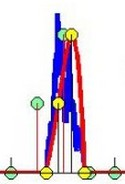
\includegraphics{analyse/sunriseadaption}
\caption{Ergebnis der Sonnenaufgangs- und Untergangsadaption}
\label{fig:sunriseadapt}
\end{wrapfigure}
An dieser Stelle sieht man zunächst das Ergebnis der Sonnenauf- und Sonnenuntergangsadaption. Wie in der \textbf{Abbildung \ref{fig:sunriseadapt}} zu erkennen, würde ohne diese Adaption die Spline Kurve durch die grünlich markierten Punkte verlaufen. Wobei der erste und letzte Punkt, den Tagesbeginn 0.00 Uhr bzw. das Tagesende 23.59 Uhr markieren. Das hieße aber, dass es Globalstrahlung den ganzen Tag über geben würde. Die von der Wetterstation gelieferten Werte müssen daher auf den Zeitraum von Sonnenaufgang- bis Sonnenuntergang, hier als gelbe Punkte auf der x-Achse dargestellt, gemappt werden. Das Mapping der Werte geschieht dabei in gleichen Abständen.
\begin{figure}[htbp]
\centering
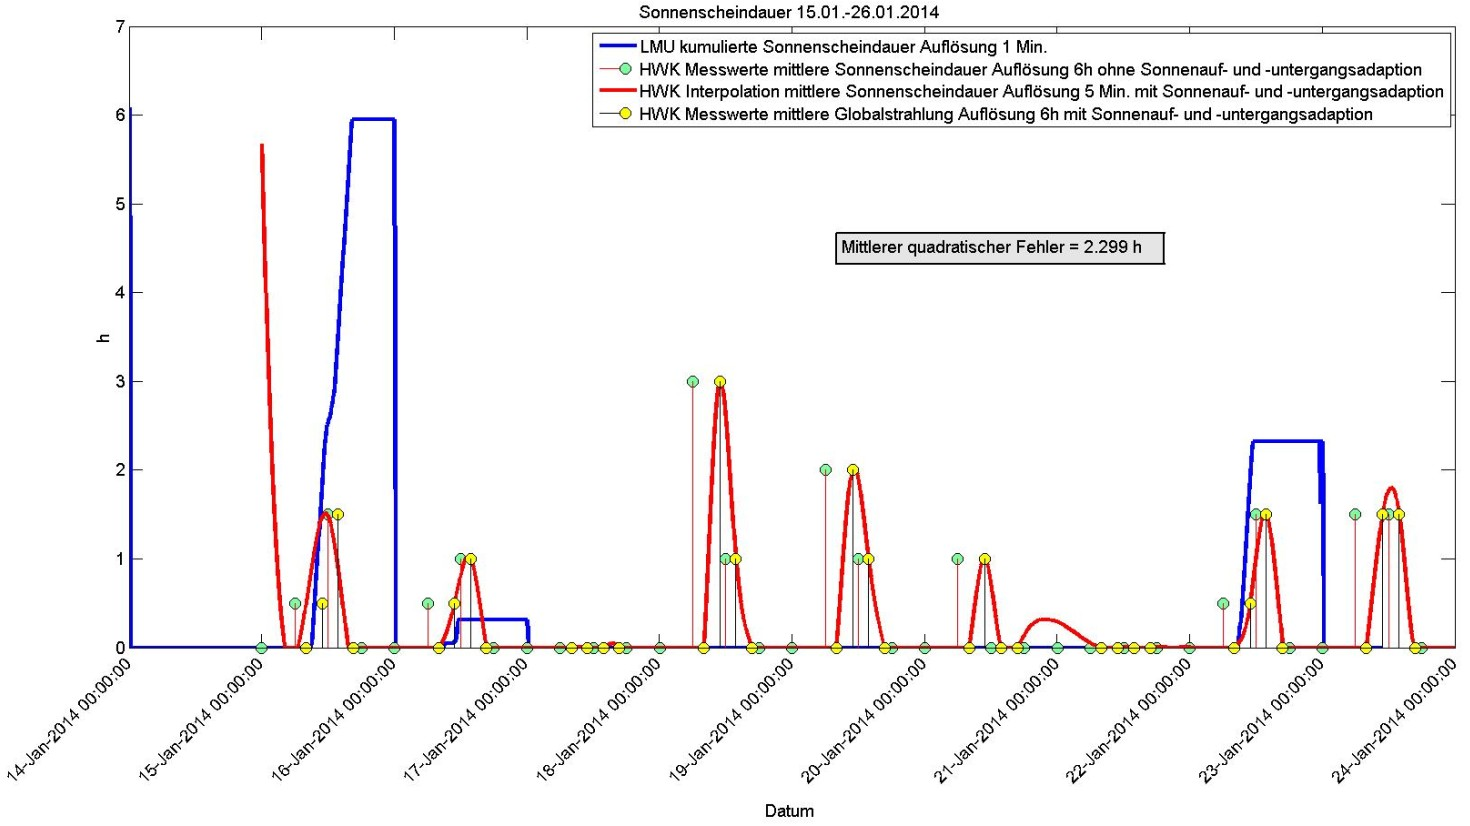
\includegraphics[width=16cm,height=10cm]{analyse/sonnensdauer2}
\caption{Vergleich der interpolierten Sonnenscheindauer mit den LMU Wetterdaten, Beobachtungsintervall 15.-24.01.2014}
\label{fig:sonnensdauer}
\end{figure}

Bei der Sonnenscheindauer gibt es Diskrepanzen zwischen den Daten der LMU und denen der Wetterstation. Während die LMU keinen Sonnenschein ausweist, registriert die Wetterstation beispielsweise vom 18.01. bis einschließlich 20.01.2014 positive Werte. Dies kann an der Definition des Sonnenscheins liegen. In der Spezifikation der Station wird dann von Sonnenschein gesprochen, wenn die Globalstrahlung mehr als 120W/m² beträgt. Nach Rücksprache mit Herrn Lösslein von der LMU, wird bei den LMU Daten ebenfalls dieses Kriterium angewandt \cite{loesslein}. Wie im Gespräch mit Herrn Volkhardt von der Firma HKW GmbH zu ermitteln war, gibt es die Möglichkeit, solche Abweichungen beim Qualitätsmanagement des Wetterdienstes über die Firma HKW einzureichen \cite{TelHKW}. Da die Werte der LMU kumuliert sind, die der Wetterstation jedoch nicht, wird hier zum Vergleich der Prognosegüte nicht der RMSE verwendet. Es wird lediglich über die MATLAB Funktion \textsf{trapz} die Fläche unter den Spline-Kurven angenähert und dann mit dem maximalen Wert der LMU Daten verglichen. Hierbei fällt auf, dass die Prognose vom 22.01. näher an den realen Daten lag, als der dann tatsächlich vorliegende Wert der Wetterstation an diesem Tag. Für ein besseres Bild der Prognosegüte müssen mehr Daten ausgewertet werden.  
\begin{table}[t]
\caption{Absolute Abweichung der Sonnenscheindauer von den LMU Wetterdaten in Stunden, Beobachtungsintervall 15.-24.01.2014}
\rowcolors{1}{cyan}{white}
{
\setlength{\extrarowheight}{0.1cm}
\begin{tabular}{| c | c | c | c | c | c | c | c | p{1cm} |}
\hline
\textbf{\parbox[t]{2.7cm}{Abrufdatum\\Intervall\\18.00-24.00 Uhr}} & \textbf{16.01.} & \textbf{17.01.} & \textbf{18.01.} & \textbf{19.01.} & \textbf{20.01.} & \textbf{21.01.} & \textbf{22.01.} & \textbf{23.01.} \\[1cm]
\hline \hline
\hiderowcolors
16.01.2014 & \cellcolor{red!25}2.66  & \cellcolor{green!25}0.11 &  &  &  &  &  & \\
17.01.2014 &  	    & \cellcolor{red!25}0.03 & \cellcolor{green!25}8.22 &  &  &  &  & \\
18.01.2014 &		& 		& \cellcolor{red!25}7.45 & \cellcolor{green!25}6.04 &  &  &  & \\
19.01.2014 &  	    &  	    & 	     & \cellcolor{red!25}5.49 & \cellcolor{green!25}2.54 &  &  &  \\ 
20.01.2014 &        &       &        &        & \cellcolor{red!25}2.18 & \cellcolor{green!25}0.08 &  & \\
21.01.2014 &        & 	    & 	     & 		  &  	   & \cellcolor{red!25}0.08 & \cellcolor{green!25}1.12 & \\
22.01.2014 &        & 	    & 	     & 		  &  	   & 						  & \cellcolor{red!25}1.83 & \cellcolor{green!25}4.21\\
\hline
\parbox[t]{2.7cm}{prozentuale\\Abweichung\\der realen HKW Werte von\\ der Prognose}& & -73.0 & -9.4 & -9.1 & -14.1 & 0.0 & +63.0 & \\  
\hline
\end{tabular}
}
\label{tab:proggsd}
\end{table}
%Sonnenscheindauerende
\section{Globalstrahlung}
%Globalstrahlunganfang
Beim Vergleich der Globalstrahlung in \textbf{Abbildung \ref{fig:globalstr}} bietet sich ein geteiltes Bild. Im Bereich niedriger Globalstrahlung ($<$ 200W/m²) befindet sich der RMSE auf einem recht akzeptablen Niveau (siehe \textbf{Tabelle \ref{tab:proggglob}}). Dies ändert sich jedoch bei großen Ausschlägen nach oben, wie sie am 22. und 23.01.2014 zu beobachten sind. Betrachtet man den 23.01. genauer, so lagen die Werte bei 75 und 100 W/m² für das Intervall von 6 Uhr bis 12 Uhr bzw. 12 bis 18 Uhr. Der Sonnenaufgang und der -untergang für diese Jahreszeit findet gegen 8 Uhr und 16.45 Uhr statt. D.h. ca. 250 W/m² fehlen dem eigentlich relevanten Intervall in dem die Sonne scheint. Verteilt man diese Energie auf die verbleibenden 9 Stunden, würde das die Kurve um ca. 28 W/m² nach oben verschieben. Die Daten der LMU erreichen an diesem Tag Spitzenwerte bis über 400 W/m². Die Werte fallen auch nicht nennenswert unter 100W/m², so dass davon ausgegangen werden kann, dass der mittlere Wert der LMU Daten höher liegt. Auch hier müsste man evtl. die Daten dem Anbieter der Wetterstation übergeben und vom Wetterdienst überprüfen lassen.   
\begin{figure}[htbp]
\centering
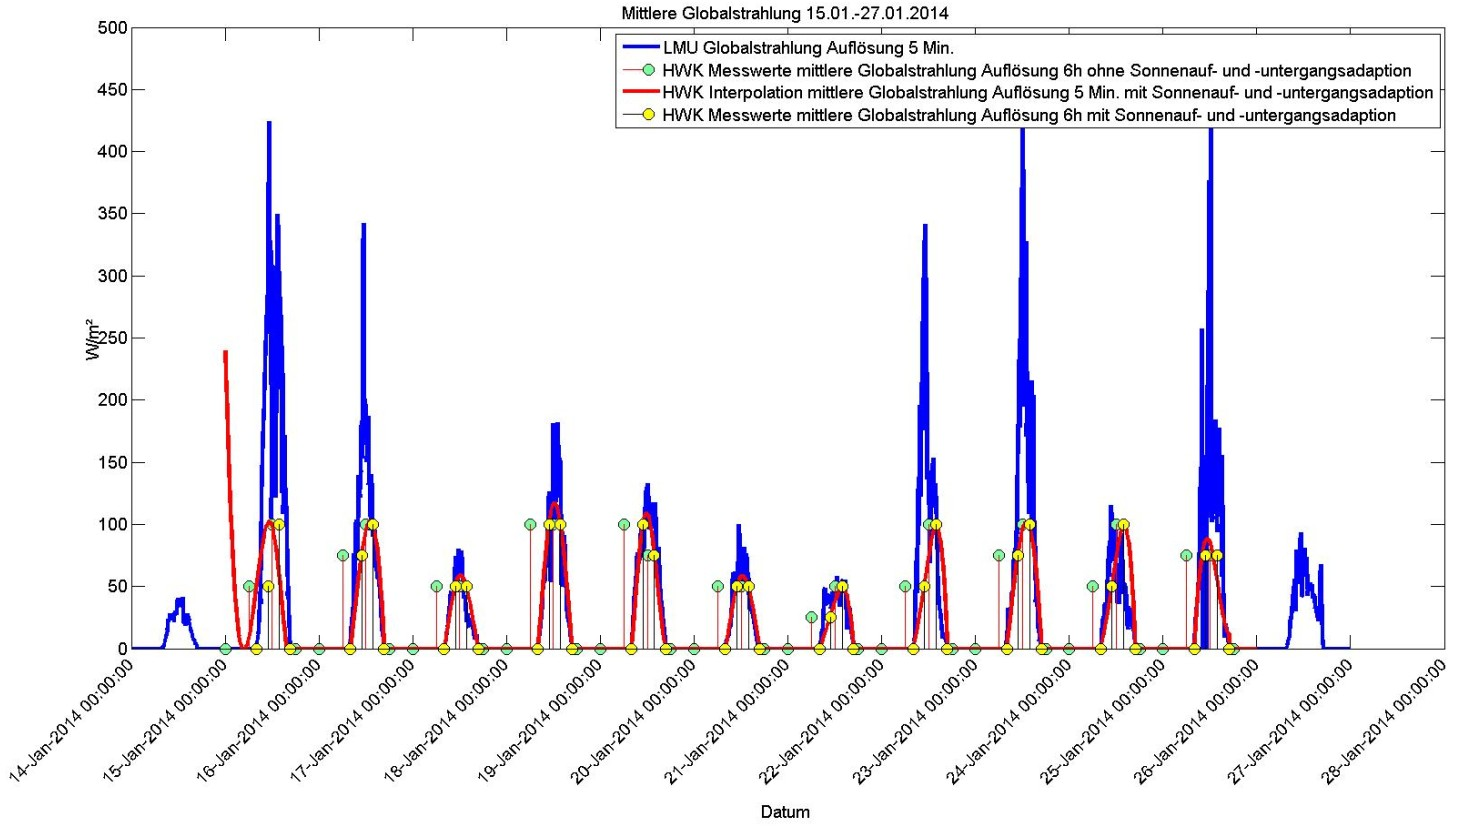
\includegraphics[width=16cm,height=10cm]{analyse/globalstr2}
\caption{Vergleich der interpolierten Globalstrahlung mit den LMU Wetterdaten, Beobachtungsintervall 15.-24.01.2014}
\label{fig:globalstr}
\end{figure}
%Text
\begin{table}[t]
\caption{RMSE der Globalstrahlung in W/m²}
\rowcolors{1}{cyan}{white}
{
\setlength{\extrarowheight}{0.1cm}
\begin{tabular}{| c | c | c | c | c | c | c | c  | p{1.5cm} |}
\hline
\textbf{\parbox[t]{2.7cm}{Abrufdatum\\Intervall\\18.00-24.00 Uhr}} & \textbf{16.01.} & \textbf{17.01.} & \textbf{18.01.} & \textbf{19.01.} & \textbf{20.01.} & \textbf{21.01.} & \textbf{22.01.} & \textbf{23.01.} \\[1cm]
\hline \hline
\hiderowcolors
16.01.2014 & \cellcolor{red!25}38.11  & \cellcolor{green!25}5.10 &  &  &  &  &  & \\
17.01.2014 &  	   & \cellcolor{red!25}6.78 & \cellcolor{green!25}22.18 &  &  &  &  & \\
18.01.2014 &	   & 		& \cellcolor{red!25}16.37 & \cellcolor{green!25}13.22 &  &  &  & \\
19.01.2014 &  	   &  	    & 	     & \cellcolor{red!25}11.27 & \cellcolor{green!25}7.47 &  &  & \\ 
20.01.2014 &       &        &        &        & \cellcolor{red!25}7.36 & \cellcolor{green!25}12.09 &  & \\
21.01.2014 &       & 	    & 	     & 		  &  	   & \cellcolor{red!25}7.97 & \cellcolor{green!25}49.76 & \\
22.01.2014 &       & 	    & 	     & 		  &  	   & 						  & \cellcolor{red!25}59.81   & \cellcolor{green!25}68.55 \\
\hline
\parbox[t]{2.7cm}{prozentuale\\Abweichung\\der realen HKW Werte von\\ der Prognose}& & +32.9 & -26.2 & -14.8 & -1.5 & -34.0 & +20.2 & \\
\hline
\end{tabular}
}
\label{tab:proggglob}
\end{table}
%Globalstrahlungende
\section{Niederschlagsmenge}
%Niederschlaganfang
Die Niederschlagsmenge wird ebenfalls wie zuvor schon die Solardaten mit einer 6 stündigen Auflösung bereit gestellt. Die Daten der LMU liegen in einer 1 Minuten Auflösung vor. Um die beiden Daten miteinander vergleichbar machen zu können, musste der HKW Wert mit einer Division durch 72 auf ein 5 Minuten Intervall gebracht und die LMU Daten auf 5 Min. gemittelt werden. Im Gegensatz zur Globalstrahlung liegen hier die mittleren Werte der Wetterstation meist über denen der LMU (siehe \textbf{Abbildung \ref{fig:niedersmenge}}). Betrachtet man den Prognoseverlauf vom 18.01. bis zum aktuellen Wert am 22.01. so erwartet man eine stetige Verbesserung der Werte, da weiter in der Zukunft liegende Prognosen unsicherer sind. Das ist aber nicht der Fall (vgl. \textbf{Tabelle \ref{tab:proggns}}). Ob sich das auch über einen längeren Zeitraum hinzieht müsste mit einem größeren Datensatz überprüft werden. 
\begin{figure}[htbp]
\centering
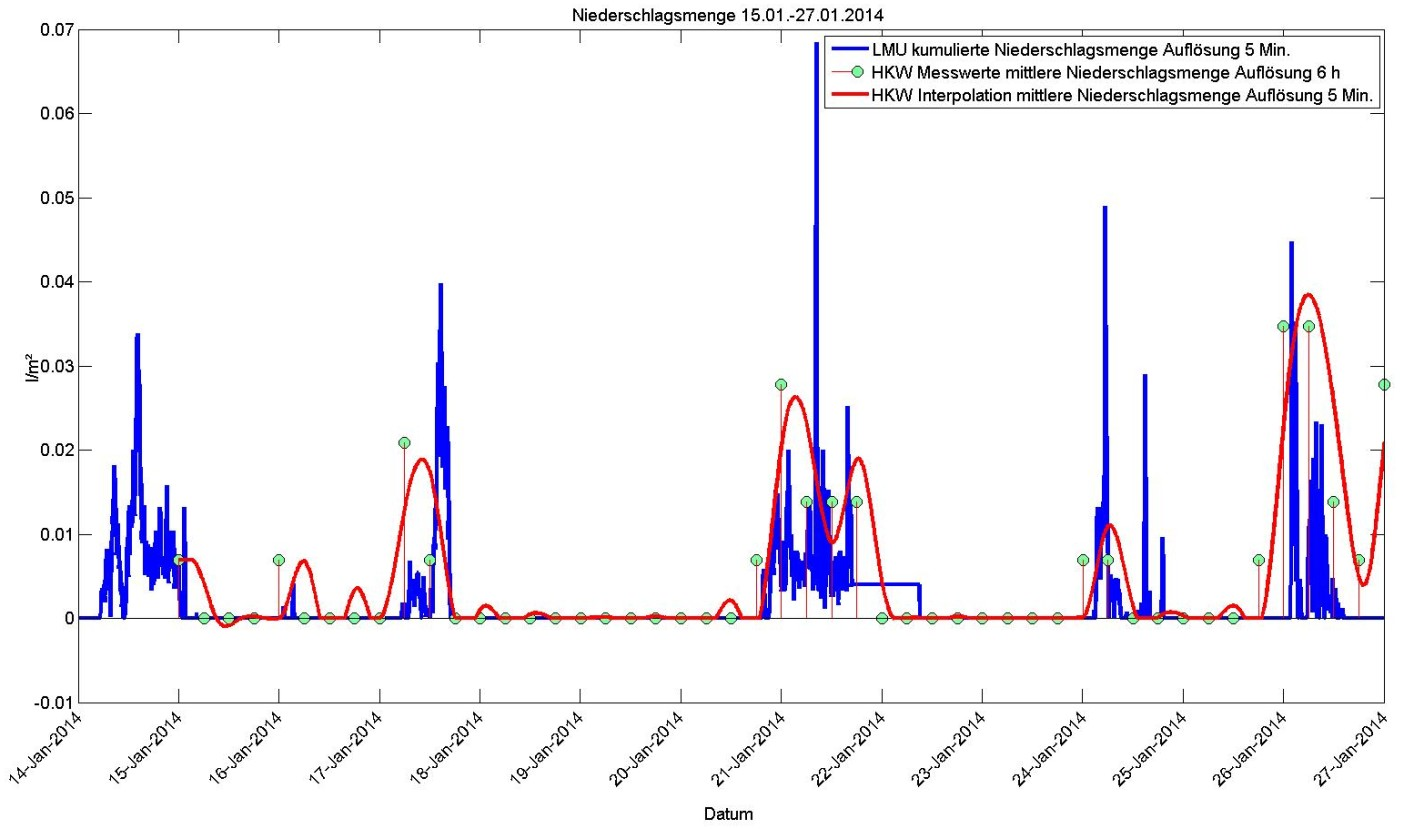
\includegraphics[width=16cm,height=10cm]{analyse/niedersmenge2}
\caption{Vergleich der interpolierten Niederschlagsmenge mit den LMU Wetterdaten, Beobachtungsintervall 15.-24.01.2014}
\label{fig:niedersmenge}
\end{figure}
\begin{table}[t]
\caption{RMSE der Niederschlagsmenge in l/m²}
\rowcolors{1}{cyan}{white}
{
\setlength{\extrarowheight}{0.1cm}
\begin{tabular}{| c | p{1cm} | p{1cm} | p{1cm} | p{1cm} | p{1cm} | p{1cm} | p{1cm} | p{1cm} | p{1cm} |}
\hline
\textbf{\parbox[t]{2.3cm}{Abrufdatum\\Intervall\\18.00-24.00 Uhr}} & \textbf{16.01.} & \textbf{17.01.} & \textbf{18.01.} & \textbf{19.01.} & \textbf{20.01.} & \textbf{21.01.} & \textbf{22.01.} & \textbf{23.01.} & \textbf{24.01.} \\[1cm]
\hline \hline
\hiderowcolors
16.01.2014 & \cellcolor{red!25}0.22 & \cellcolor{green!25}0.43 & \cellcolor{yellow!25}0.04 & 0.00 &  &  &  &  & \\
17.01.2014 &  	    & \cellcolor{red!25}0.76 & \cellcolor{green!25}0.04 & \cellcolor{yellow!25}0.01 & 0.70 &  &  &  & \\
18.01.2014 &	    & 		& \cellcolor{red!25}0.04 & \cellcolor{green!25}0.03 & \cellcolor{yellow!25}0.82 & 1.14 &  &  & \\
19.01.2014 &  	    &  	    & 	     & \cellcolor{red!25}0.01 & \cellcolor{green!25}0.27 & \cellcolor{yellow!25}0.98 & 0.27 &  & \\ 
21.01.2014 &        &       &        &        & \cellcolor{red!25}0.38 & \cellcolor{green!25}1.40 & \cellcolor{yellow!25}0.07 & 0.23 & \\
22.01.2014 &        & 	    & 	     & 		  &  	   & \cellcolor{red!25}1.27 & \cellcolor{green!25}0.05 & \cellcolor{yellow!25}0.03 & 0.66 \\
\hline
\multirow{5}{2.3cm}{prozentuale Abweichung der realen HKW Werte von der Prognose} &  & +76.7 & 0.0 & - &  &  &  &  & \\
&  &  & 0.0 & +300 & +17.1 &  &  &  & \\
&  &  & 	& -66.7 & -67.1 & -14.3 &  &  & \\ 
&  &  &     &       & +40.7 & +42.9 & -74.1 &  & \\
&  &  & 	& 		&  	    & -9.3  & -28.6 & -87.0 & \\
\hline
\end{tabular}
}
\label{tab:proggns}
\end{table}
%Niederschlagende
\section{Windstärke}
%Windanfang
\begin{figure}[htbp]
\centering
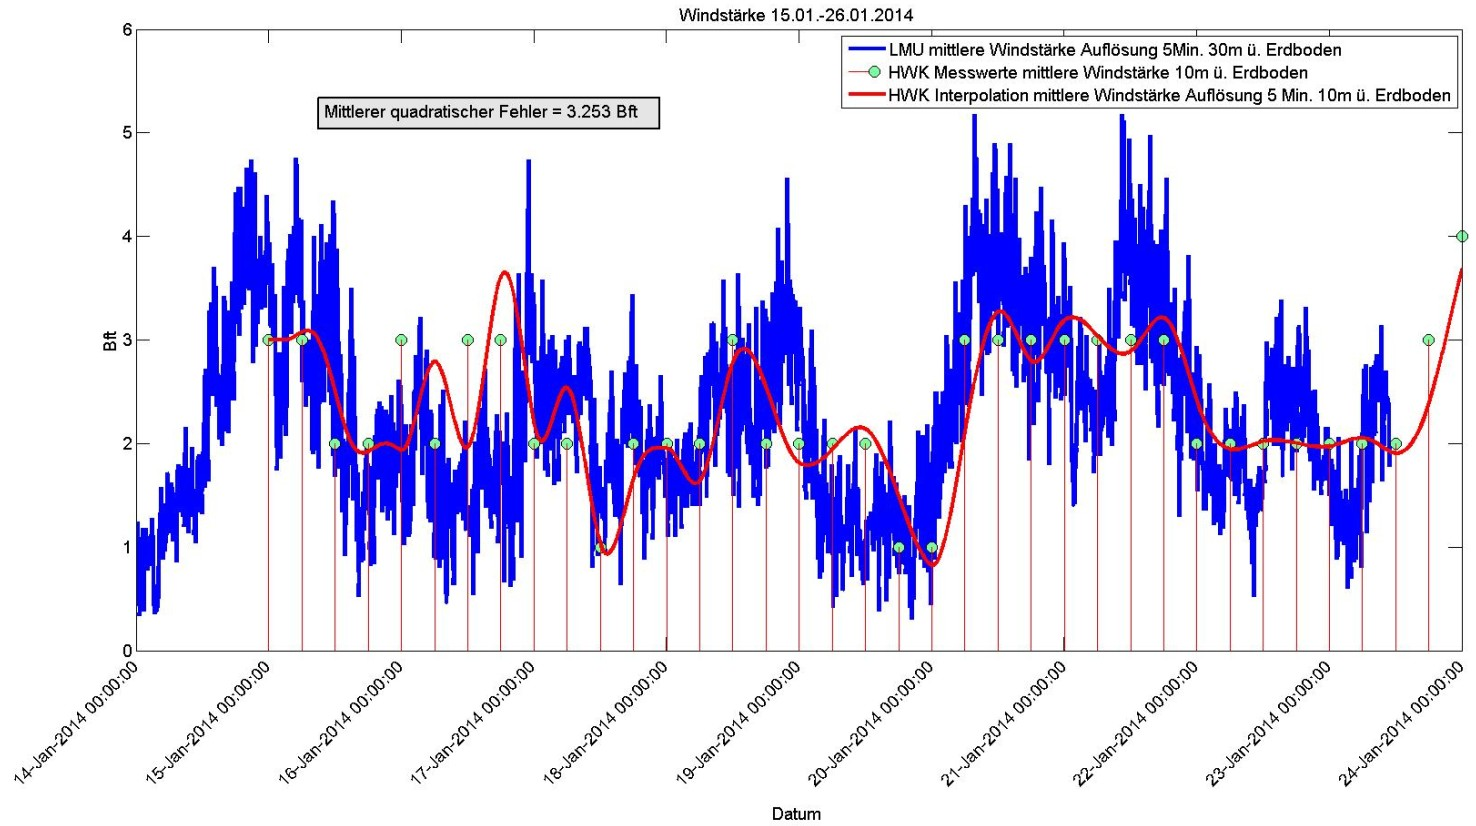
\includegraphics[width=16cm,height=10cm]{analyse/windstaerke2}
\caption{Vergleich der interpolierten Windstaerke mit den LMU Wetterdaten, Beobachtungsintervall 15.-24.01.2014}
\label{fig:windstaerke}
\end{figure}
\begin{table}[t]
\caption{RMSE der Windstärke in Bft}
\rowcolors{1}{cyan}{white}
{
\setlength{\extrarowheight}{0.1cm}
\begin{tabular}{| c | p{1cm} | p{1cm} | p{1cm} | p{1cm} | p{1cm} | p{1cm} | p{1cm} | p{1cm} | p{1cm} |}
\hline
\textbf{\parbox[t]{2.3cm}{Abrufdatum\\Intervall\\18.00-24.00 Uhr}} & \textbf{16.01.} & \textbf{17.01.} & \textbf{18.01.} & \textbf{19.01.} & \textbf{20.01.} & \textbf{21.01.} & \textbf{22.01.} & \textbf{23.01.} & \textbf{24.01.} \\[1cm]
\hline \hline
\hiderowcolors
16.01.2014 & \cellcolor{red!25}1.23 & \cellcolor{green!25}0.66 & \cellcolor{yellow!25}0.81 & 0.76 &  &  &  &  & \\
17.01.2014 &  	   & \cellcolor{red!25}0.72 & \cellcolor{green!25}0.87 & \cellcolor{yellow!25}0.55 & 0.91 &  &  &  & \\
18.01.2014 &		   & 		& \cellcolor{red!25}0.78 & \cellcolor{green!25}0.72 & \cellcolor{yellow!25}1.32 & 0.91 &  &  & \\
19.01.2014 &  	   &  	    & 	     & \cellcolor{red!25}0.77 & \cellcolor{green!25}1.37 & \cellcolor{yellow!25}0.89 & 0.61 &  & \\ 
21.01.2014 &        &        &        &        & \cellcolor{red!25}1.07 & \cellcolor{green!25}0.91 & \cellcolor{yellow!25}0.65 & 0.94 & \\
22.01.2014 &        & 	    & 	     & 		  &  	   & \cellcolor{red!25}0.92 & \cellcolor{green!25}0.62 & \cellcolor{yellow!25}0.94 & 1.05 \\
\hline
\multirow{5}{2.3cm}{prozentuale Abweichung der realen HKW Werte von der Prognose} &  	   & +9.1 & +7.4 & -27.6 &  &  &  &  & \\
 &		   & 		& -10.3 & +30.9 & +45.1 &  &  &  & \\
 &  	   &  	    & 	     & +6.9 & +3.8 & -2.2 &  &  & \\ 
 &        &        &        &        & -21.9 & +2.2 & +6.6 &  & \\
 &        & 	    & 	     & 		  &  	   & +1.1 & -4.6 & 0.0 & \\ 
\hline
\end{tabular}
}
\label{tab:proggwind}
\end{table}
 
Die Windstärkedaten der LMU sind mit einer Auflösung von einer Minute äußerst genau. was sich in den häufigen Ausschlägen widerspiegelt. Dennoch folgt der Graph der interpolierten Daten in der \textbf{Abbildung \ref{fig:windstaerke}} relativ gut dem Gesamtverlauf. Da die Windstärke in einer Höhe von 30m an der LMU gemessen wird. lassen sich evtl. die Abweichungen von einem Bft erklären. Die Daten der Wetterstation beziehen sich auf 10m über dem Erdboden. 

Geht man zum Beispiel von einer Stärke von 3 Bft auf 10m Höhe aus. dann kann man über das logarithmische Grenzschichtprofil die Windstärke in 30m Höhe abschätzen. Die Formel hierzu lautet: \(v(30m) = v(10m)*\frac{ln(\frac{30m-0}{2})}{ln(\frac{10m-0}{2})}\). Mit einer Geländeklasse. die einem Stadtkern entspricht. ergibt sich bei einer Geschwindigkeit von 4.4m/s für v(10m) und keinem Versatz der Grenzschicht durch Hindernisse ein Wert von 7.4m/s. der ungefähr einem Bft mehr entspricht. \cite{GrenzProf}

Wie gut nun die Prognosewerte sind. darüber lässt sich wie vorhin erwähnt eine Aussage mit dem Root Mean Squared Error (RMSE) treffen \cite{DWD}. Dieser stellt die Standardabweichung der Differenzen zwischen Prognose- und Beobachtungswert dar. Der Deutsche Wetterdienst empfiehlt in seiner Broschüre keine größere Abweichung als 1 Bft für eine gute Prognose \cite{DWD}. Die nachfolgende \textbf{Tabelle \ref{tab:proggwind}} stellt jeweils den RMSE für unterschiedliche Abrufdaten dar. Wie man in der Tabelle erkennen kann. wird dieses Qualitätsmerkmal weitgehend eingehalten. 
%Windende 
\section{Mittlere Lufttemperatur}
%Luftanfang 
Die mittlere Lufttemperatur wird mit einer 1 stündigen Auflösung an die Wetterstation übertragen. Es ist deshalb davon auszugehen. dass diese Daten verglichen mit den Daten der LMU weniger große Diskrepanzen aufweisen. Betrachtet man die \textbf{Abbildung \ref{fig:mittlufttemp}} so vermittelt diese. einen die vorige Aussage bestätigenden Eindruck. Auffallend jedoch ist der teilweise Versatz der Datenpunkte nach unten. Ein Blick auf den RMSE in der \textbf{Tabelle \ref{tab:progglufttemp}} zeigt. dass es sich hierbei meist um 1 bis 2 $^\circ$C bei den tagesaktuellen Daten und 1 bis 3.5 $^\circ$C bei den Prognosedaten handelt. Ein Grund für diese eher einseitige Abweichung nach unten könnte ein unterschiedlicher Standort der beiden Wetterstationen sein. Die LMU Wetterstation befindet sich direkt im Stadtzentrum. Bewegt man sich hin zu den Randbezirken Münchens. kann die Temperatur um bis zu 6 $^\circ$C abfallen \cite{stadtklima}. Auch hier ist der Verlauf der Prognoseentwicklung nicht immer der. den man erwarten würde. Nimmt man zum Beispiel den 19. Januar so war die Prognose am 16.01.2014 für diesen Tag besser als die beiden Darauffolgenden. die weniger weit in die Zukunft reichen. Hinsichtlich der Prognosegüte kann man unter Berücksichtigung des vermutlichen Standortunterschieds gem. dem DWD von einer guten Vorhersage ausgehen. Dieser gibt hierfür einen Grenzwert von 2.5 $^\circ$C (RMSE) vor \cite{DWD}. Um diesen evtl. standortabhängigen Temperatureffekt zu korrigieren. bietet es sich vielleicht an. den in der Wetterstation integrierten Temperatursensor mitzuverwenden. Eine historische Auswertung der Daten und ein daraus ermittelter Korrekturfaktor könnten den Offset ausgleichen.        
\begin{figure}[h]
\centering
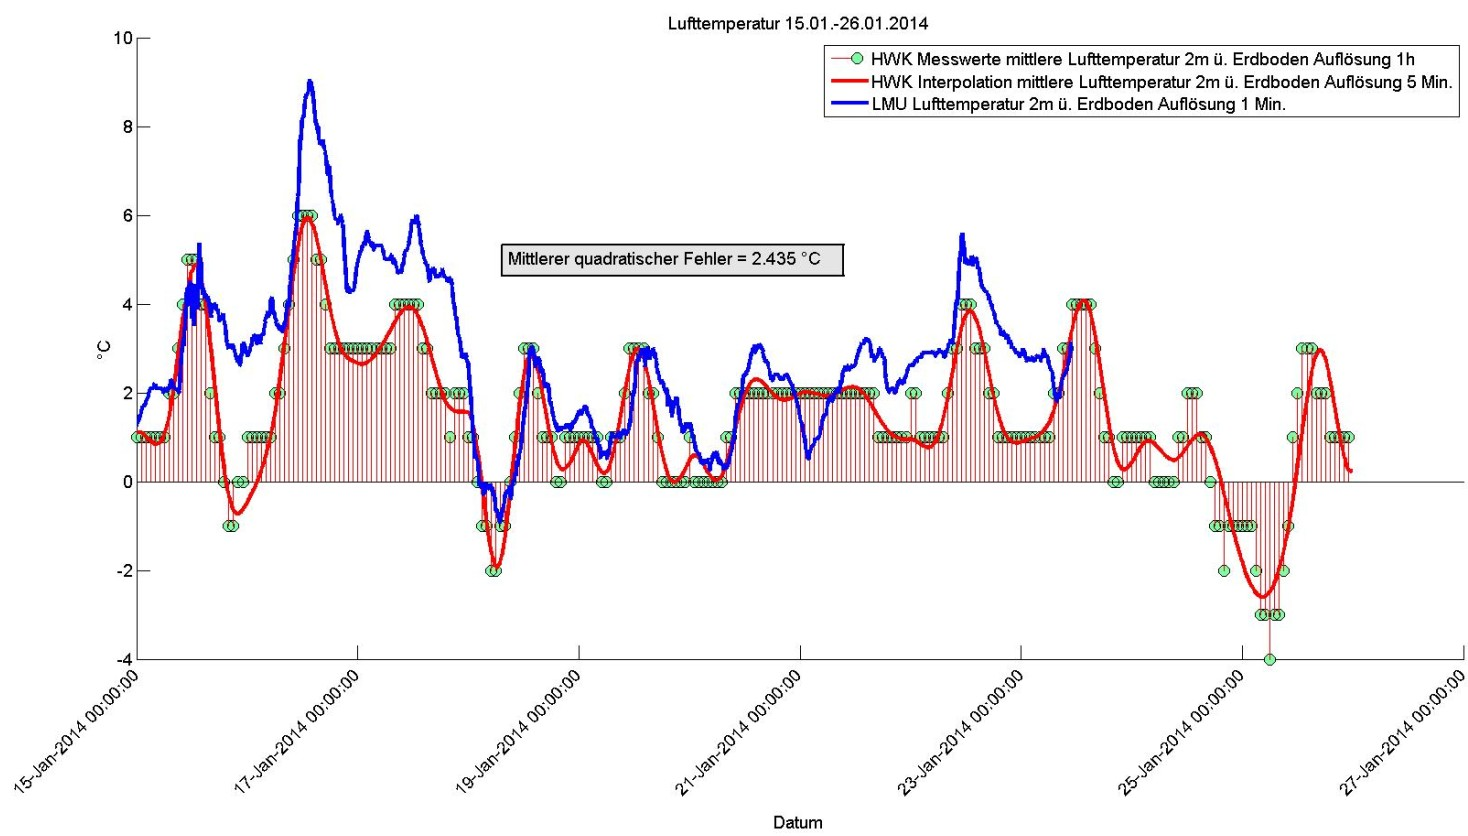
\includegraphics[width=16cm,height=10cm]{analyse/mittlufttemp2}
\caption{Vergleich der interpolierten mittleren Lufttemperatur mit den LMU Wetterdaten, Beobachtungsintervall 15.-24.01.2014}
\label{fig:mittlufttemp}
\end{figure}
\begin{table}[h]
\caption{RMSE der mittleren Lufttemperatur in $^\circ$C}
\rowcolors{1}{cyan}{white}
{
\setlength{\extrarowheight}{0.1cm}
\begin{tabular}{| c | p{1cm} | p{1cm} | p{1cm} | p{1cm} | p{1cm} | p{1cm} | p{1cm} | p{1cm} | p{1cm} |}
\hline
\textbf{\parbox[t]{2.3cm}{Abrufdatum\\Intervall\\18.00-24.00 Uhr}} & \textbf{16.01.} & \textbf{17.01.} & \textbf{18.01.} & \textbf{19.01.} & \textbf{20.01.} & \textbf{21.01.} & \textbf{22.01.} & \textbf{23.01.} & \textbf{24.01.} \\[1cm]
\hline \hline
\hiderowcolors
16.01.2014 & \cellcolor{red!25}2.30 & \cellcolor{green!25}2.65 & \cellcolor{yellow!25}2.03 & 1.35 &  &  &  &  & \\
17.01.2014 &  	   & \cellcolor{red!25}2.04 & \cellcolor{green!25}2.81 & \cellcolor{yellow!25}1.90 & 0.77 &  &  &  & \\
18.01.2014 &		   & 		& \cellcolor{red!25}0.81 & \cellcolor{green!25}2.07 & \cellcolor{yellow!25}1.13 & 1.08 &  &  & \\
19.01.2014 &  	   &  	    & 	     & \cellcolor{red!25}0.99 & \cellcolor{green!25}0.58 & \cellcolor{yellow!25}0.61 & 2.84 &  & \\ 
20.01.2014 &        &        &        &        & \cellcolor{red!25}0.53 & \cellcolor{green!25}1.08 & \cellcolor{yellow!25}3.21 & 3.66 & \\
21.01.2014 &        & 	    & 	     & 		  &  	   & \cellcolor{red!25}1.03 & \cellcolor{green!25}3.01 & \cellcolor{yellow!25}2.77 & 2.76 \\
\hline
\multirow{5}{2.3cm}{prozentuale Abweichung der realen HKW Werte von der Prognose} &  	   & -23.0 & +38.4 & +40.7 &  &  &  &  & \\
 &		   & 		& -71.2 & +9.0 & +46.8 &  &  &  & \\
 &  	   &  	    & 	     & -52.2 & -48.7 & -43.5 &  &  & \\ 
 &        &        &        &        & -8.6 & +77.1 & +13.0 &  & \\
 &        & 	    & 	     & 		  &  	   & -4.6 & -6.2 & -24.3 & \\
\hline
\end{tabular}
}
\label{tab:progglufttemp}
\end{table}
%Luftende
\part{Schluss}
\chapter{Zusammenfassung und Ausblick}
Aufgabe war es die Daten einer Wetterstation wiederholt auszulesen und für die weitere Verarbeitung zu interpolieren bzw. abzuspeichern. Für die Entwicklung des Programmcodes waren das Wissen um die MODBUS- und Wetterstationsspezifikation von entscheidender Bedeutung. Ausgehend von diesen Informationen konnte in einem ersten Schritt in einer virtuellen Umgebung die Kommunikation über die serielle Schnittstelle getestet werden. Mit den nun bekannten Funktionalitäten konnte der weitere Programmaufbau für das mehrmalige Senden und Auslesen von MODBUS-Nachrichten implementiert werden. Als kleine Schwierigkeit gestaltete sich der Aufbau der kontinuierlichen Zeitreihe, da die Grunddaten selbst in einer unterschiedlichen Auflösung vorliegen. Aber auch dieses Problem konnte letztendlich gelöst werden. Nachdem die ersten Ergebnisse vorlagen und mit den Daten des metereologischen Instituts der LMU verglichen wurden, ergaben sich neue Verbesserungsmöglichkeiten. Im Bereich der Solarleistung wurden daraufhin die Daten der Wetterstation auf den Tagesgang der Sonne gemappt. Ein nachträglicher Vergleich bestätigte den Erfolg dieser Maßnahme deutlich. Trotz der guten Datenaufbereitung gibt es noch Verbesserungspotential. Bezogen auf die Temperaturen kann aufbauend auf historische Daten, die vom lokalen Temperatursensor stammen, ein Ausgleichsfaktor bestimmt werden, welcher die Prognosedaten an die tatsächlich vor Ort vorherrschenden Temperaturen anpasst. Für einen Test über einen längeren Zeitraum als einer Woche war in dieser Arbeit leider keine Zeit. Daher wäre es zu empfehlen diesen noch durchzuführen. Der in dieser Arbeit ausgegebene Luftdruck bezieht sich auf das Niveau des Meeresspiegels. Soll ein ortsabhängiger Luftdruck in den Daten gespeichert werden, so müssen die jeweiligen Höhen der Wetterregionen und die barometrische Höhenformel mit in den Programmcode integriert werden. Die Sonnenauf- und -untergangsadaption ist bis jetzt nur für deutsche Städte vorgesehen. Sollen andere europäische Wetterregionen abgerufen werden, so müssen die Längen- und Breitengrade im Code ergänzt werden.     
\appendix
\renewcommand*{\appendixpagename}{Anhang}
\renewcommand*{\appendixtocname}{Anhang}
\appendixpage 
\addappheadtotoc
\chapter{Aufbau der Wetterstation} 
%\begin{figure}[h]
%\centering
%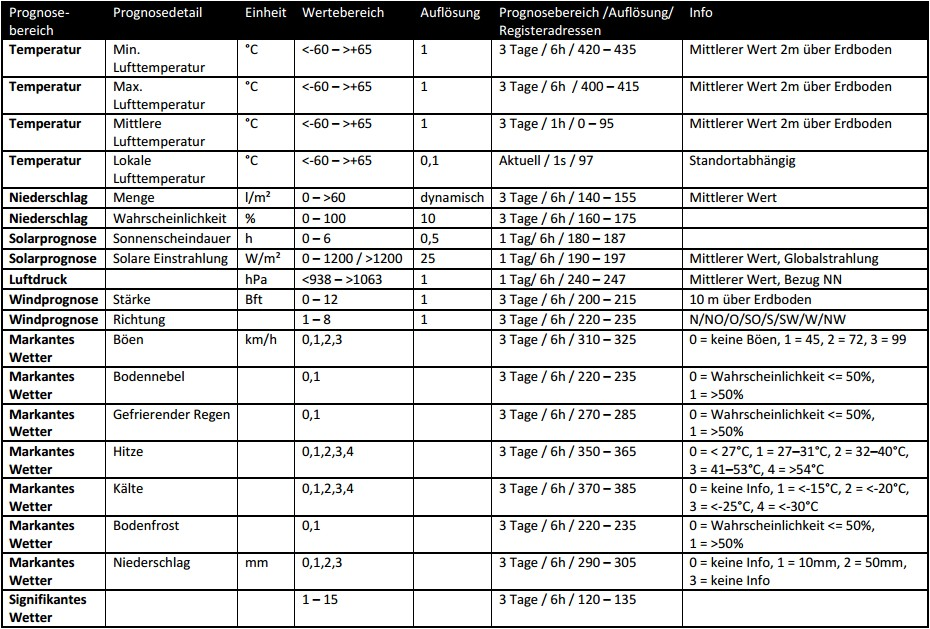
\includegraphics[scale=0.65]{weatherstation/TabDatenstruktur}
%\caption{Detailierte Datenstruktur der Wetterstation\cite[S. 17-26]{HKWDoc}}
%\label{fig:detaildatenstruktur}
%\end{figure}
\begin{table}[!b]
\rotatebox{90}{
\begin{minipage}[!b]{\textwidth}
\resizebox{18.9cm}{!}{ 
\rowcolors{1}{cyan}{white}
{
\setlength{\extrarowheight}{0.1cm}
\begin{tabular}[!b]{| p{2.5cm} | l | l | l | l | l | l | l | p{6.4cm} |}
\hline
\textbf{\parbox[t]{2.7cm}{Prognose-\\Bereich}} & \textbf{Prognosedetail} & \textbf{\parbox[t]{1.2cm}{Ein-\\heit}} & \textbf{Wertebereich} & \textbf{\parbox[t]{1.7cm}{Auf-\\lösung}} & \textbf{\parbox[t]{1.95cm}{Prognose-\\intervall}} & \textbf{\parbox[t]{1.9cm}{zeitliche\\Auflösung}} & \textbf{\parbox[t]{1.9cm}{Register-\\adresse}} & \textbf{Info}\\[1cm]
%\textbf{\parbox[t]{2cm}{Prognose-\\bereich}} & \textbf{Prognosedetail} & \textbf{Einheit} & \textbf{Wertebereich} & \textbf{Aufloesung} & \textbf{Prognoseintervall} & \textbf{zeitliche Aufloesung} & \textbf{Registeradresse} & \textbf{Info}\\[1cm]
\hline \hline
\hiderowcolors
Temperatur & Min. Lufttemperatur & $^\circ$C &  $<-60$ bis $>65$ & 1 & 3 Tage & 6h & 420 - 435 & Mittlerer Wert 2m über Erdboden\\
Temperatur & Max. Lufttemperatur & $^\circ$C &  $<-60$ bis $>65$ & 1 & 3 Tage & 6h & 400 - 415 & Mittlerer Wert 2m über Erdboden\\
Temperatur & Mittlere Lufttemperatur & $^\circ$C &  $<-60$ bis $>65$ & 1 & 3 Tage & 1h & 000 - 095 & Mittlerer Wert 2m über Erdboden\\
Temperatur & Lokale Lufttemperatur & $^\circ$C &  $<-60$ bis $>65$ & 1 & Aktuell & 1s & 097 & Standortabhängig\\
Niederschlag & Menge & l/m$^2$ &  0-60 & dyn. & 3 Tage & 6h & 140 - 155 & Mittlerer Wert\\
Niederschlag & Wahrscheinlichkeit & \% &  0 - 100 & 10 & 3 Tage & 6h & 160 - 175 & \\
Solarprognose & Sonnenscheindauer & h &  0 - 6 & 1 & 1 Tag & 6h & 180 - 187 & Mittlerer Wert\\
Solarprognose & Solare Einstrahlung & W/m$^2$ &  0 – 1200/$>1200$ & 25 & 1 Tag & 6h & 190 - 197 & Mittlerer Wert Globalstrahlung\\
Luftdruck & Min. Lufttemperatur & hPa &  $<938$ – $>1063$ & 1 & 1 Tag & 6h & 240 - 247 & Mittlerer Wert bezogen auf NN\\
Windprognose & Stärke & Bft &  0 - 12 & 1 & 3 Tage & 6h & 200 - 215 & Mittlerer Wert 10m über Erdboden\\
Windprognose & Richtung &  &  1 - 8 & 1 & 3 Tage & 6h & 220 - 235 & N/NO/O/SO/S/SW/W/NW\\
Markantes Wetter & Böen &  &  0,1,2,3 & 1 & 3 Tage & 6h & 310 - 325 & 0=keine Böen, 1=45km/h, 2=72km/h, 3=99km/h \\
Markantes Wetter & Bodennebel &  & 0,1 & 1 & 3 Tage & 6h & 250 - 265 & 0=Wahrscheinlichkeit$<=$50\%, 1=$>$50\%\\
Markantes Wetter & Gefrierender Regen &  & 0,1 & 1 & 3 Tage & 6h & 270 - 285 & 0=Wahrscheinlichkeit$<=$50\%,1=$>$50\%\\
Markantes Wetter & Hitze & $^\circ$C &  0,1,2,3,4 & 1 & 3 Tage & 6h & 350 - 365 & 0=$<$27$^\circ$C, 1=27–31$^\circ$C, 2=32–40$^\circ$C, 3=41–53$^\circ$C, 4=$>$54$^\circ$C\\
Markantes Wetter & Kälte & $^\circ$C &  0,1,2,3,4 & 1 & 3 Tage & 6h & 370 - 385 & 0=keine Info, 1=$<$-15$^\circ$C, 2=$<$-20$^\circ$C, 3=$<$-25$^\circ$C, 4=$<$-30$^\circ$C\\
Markantes Wetter & Bodenfrost &  &  0,1 & 1 & 3 Tage & 6h & 290 - 305 & 0=Wahrscheinlichkeit$<=$50\%, 1=$>$50\%\\
Markantes Wetter & Niederschlag &  &  0,1,2,3 & 1 & 3 Tage & 6h & 330 - 345 & 0=keine Info, 1=10mm, 2=50mm, 3=keine Info\\
Signifikantes Wetter &  &  & 1 - 15 & 1 & 3 Tage & 6h & 120 - 135 & 1=sonnig/klar, 2=leicht bewölkt, 3=vorwiegend bewölkt, 4=bedeckt, 5=Wärmegewitter, 6=starker Regen, 7=Schneefall, 8=Nebel, 9=Schneeregen, 10=Regenschauer, 11=leichter Regen, 12=Schneeschauer, 13=Frontengewitter, 14=Hochnebel, 15=Schneeregenschauer\\
\hline
\end{tabular}
}
}
\caption{Detailierte Datenstruktur der Wetterstation\cite[S. 17-26]{HKWDoc}}
\label{tab:detaildatenstruktur}
\end{minipage}
}
\end{table}
\FloatBarrier
\chapter{Das MODBUS Protokoll}
\begin{figure}[h]
\centering
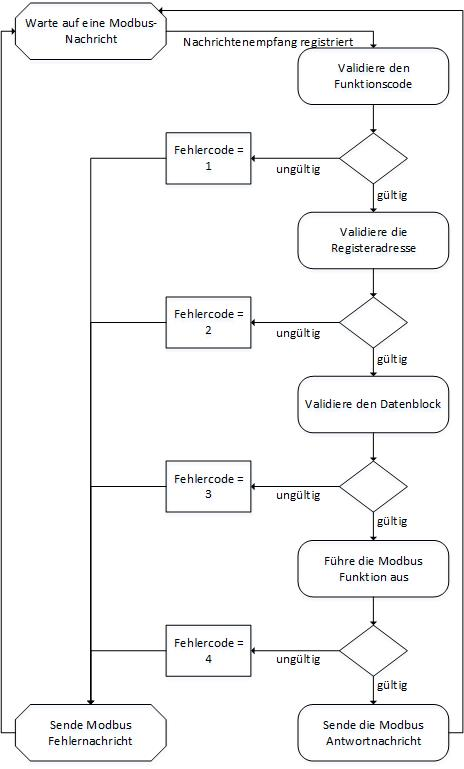
\includegraphics[scale=0.65]{modbus/modbustransdiag}
\caption{Ablaufdiagramm für die MODBUS Nachrichtenüberprüfung}
\label{fig:modbustransdiag}
\end{figure}
\newpage
\begin{figure}[hbtp]
\centering
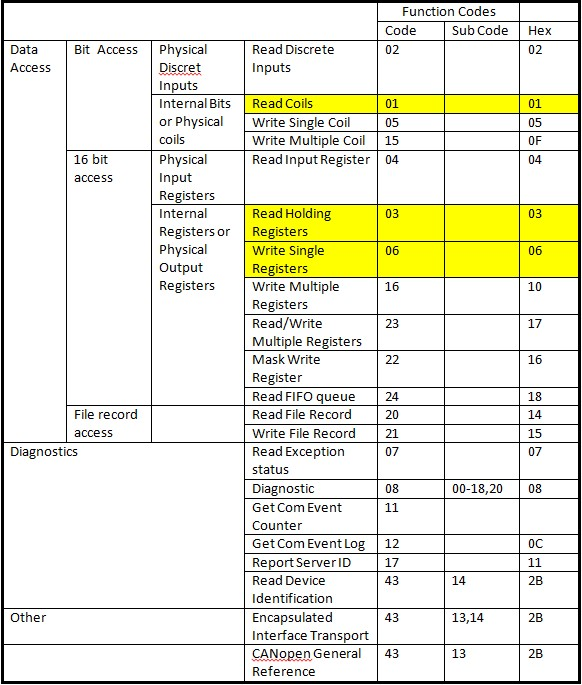
\includegraphics[scale=0.65]{modbus/fcodetab}
\caption{Übersicht der zur Verfügung stehenden Funktionscodes in MODBUS}
\label{fig:fcodetab}
\end{figure} 
\chapter{Abkürzungsverzeichnis}
\begin{acronym}
\setlength{\parskip}{0ex}
\setlength{\itemsep}{1ex}
 \acro{ADU}{Application Data Unit}
 \acro{Bft}{Beaufort}
 \acro{C}{Celsius}
 \acro{COM}{Communication}
 \acro{CRC}{Cyclic Redundancy Check}
 \acro{DWD}{Deutscher Wetterdienst}
 \acro{EMU}{Energy Management Unit}
 \acro{EV}{Electric Vehicle}
 \acro{FSK}{Frequency Shift Keying}
 \acro{GmbH}{Gesellschaft mit beschränkter Haftung}
 \acro{h}{Stunde}
 \acro{hPa}{Hektopascal}
 \acro{HEMS}{Home Energy Management System}
 \acro{H-Byte}{High-Byte}
 \acro{ID}{Identifkationsnummer}
 \acro{int8}{8 Bit-Integer}
 \acro{IP}{Internet Protocol}
 \acro{I/O}{Input/Output}
 \acro{LMU}{Ludwig-Maximilians-Universität}
 \acro{L-Byte}{Low-Byte}
 \acro{N}{Nord}
 \acro{NN}{Normal Null Meeresspiegel}
 \acro{NO}{Nordost}
 \acro{NW}{Nordwest}
 \acro{O}{Osten}
 \acro{OSI}{Open Systems Interconnection}
 \acro{PDU}{Protocol Data Unit}
 \acro{RMSE}{Root mean square error}
 \acro{RS}{Recommended Standard}
 \acro{RTU}{Remute Terminal Unit}
 \acro{rx}{Empfänger}
 \acro{TCP}{Transmission Control Protocol}
 \acro{S}{Sueden}
 \acro{SO}{Suedost}
 \acro{SW}{Suedwest}
 \acro{W}{Westen}
\end{acronym}

\bibliographystyle{unsrt} 
\bibliography{literatur} 

\end{document}


